\section{Network Topologies}\label{sec:network_topologies}
%\textcolor{blue}{The title needs to be improved!\\Explain what we are trying to do once more and how our net achieves that.}\\
\textcolor{red}{Need to introduce the optimizer we are using. Probably should do so in the beginning of the evolution section. Check entire work for ''diluted'' convolution and replace by ''dilated'' convolution.}\\
This section summarizes the results of our research, trying to find a deep learning algorithm that succeeds in detecting and classifying \gls{bns}-signals in noisy data. The goal was to not only classify the signals into the two categories ''pure noise'' and ''signal'' but also to give an estimate of the signals \gls{snr}.\\
%All software written for this work used the PyCBC software package \cite{pycbc} for any code involving gravitational wave data and the deep learning library Keras \cite{keras} to rapidly develop and test different network architectures. We used Tensorflow \cite{tensorflow} as the backend for Keras. \textcolor{red}{Should I cite the libraries here again? I did so in the introduction.}

\subsection{The Data Generating Process}\label{sec:data_generating_process}
%\textcolor{red}{Things missing: Mention training/validation split, mention that we shift the template around in the data (important for why we slide the generator in steps of 0.25s). ATTENTION!!! THE GENERATOR USED FOR THE TESTING SET CURRENTLY USES THE ANALYTIC PSD INSTEAD OF THE WHITEN FUNCTION! THIS IS DISPLAYED DIFFERENTLY IN THE TEXT! CORRECT EITHER THE GENERATOR OR THE TEXT! Take great care to carefully explain multirate filtering.}\\
%\textcolor{blue}{Explain how the data is generated (especially that it only contains gaussian noise). Explain how training/validation set are different from the testing set used in this work. Explain how we carefully chose the parameters, especially how we got the SNR-values. Also explain the mix-and-match approach, that noise can be pure or the same noise with different signals. Also the same signal can (but this isn't necessary) have multiple noise instances. The pure noise SNR was set to 4, as that is the average value for pure noise matched filtering returns. (One might want to alter this) Finally we were careful, that no noise instance or signal from the training set is used in the validation set.}\\
Training a \gls{nn} to detect and classify \gls{bns} signals requires a large set of mock data. Using the data without some processing, however, is not possible. This is due to the fact that \gls{bns} signals are more difficult to train for than \gls{bbh} signals, as they are a lot weaker and last for a longer duration\footnote{\gls{bbh} signals spend about \SI{1}{\s} within the sensitive frequency range of our detectors, whereas \gls{bns} signals can be visible in the whitened detector data for multiple tens of seconds \cite{gw170817} and when generated even last multiple hundred seconds.}. Training a \gls{nn} on data of such duration sampled at a frequency high enough to resolve the final cycles of the binary system is not feasible, as the required network would need too many trainable parameters. However, to retain most of the \gls{snr} in the data, it is not possible to crop it to only contain a small portion of the waveform. To overcome this issue note that even though \gls{bns} signals spend a long time in the sensitive region of the detectors, their frequency evolves rather slowly and starts at low values.\\
For the early inspiral phase of the signal, frequencies are around \SIrange{30}{100}{\hertz}. To resolve these frequencies, a sample rate of \SIrange{60}{200}{\hertz} is necessary. The higher sample rates are only required for the final few seconds. For these reasons we propose to represent the data using a new multi-rate approach. Using this method, the network does not receive the data at a fixed sample rate, but rather multiple inputs, each sampling parts of the signal at different rates.\\
We choose the largest window to encompass \SI{64}{\s} of data, where a signal is aligned such, that the high frequency cutoff is roughly \SI{0.5}{\s} from the end. Afterwards we chop the data into parts of duration \SI[parse-numbers=false]{2^i}{\s} and re-sample each of these parts to have a sample rate of \SI[parse-numbers=false]{2^{12-i}}{\hertz}, with $i=0,\dotsc ,6$. This way each sample rate contains exactly $4096$ samples.\\
The 7 re-sampled data segments, however, have overlaps. This is due to the fact, that the lower sample rates contain the data of the higher sample rates, e.g. the \SI{2}{\s} interval sampled at \SI{2048}{\hertz} also includes the \SI{1}{\s} interval sampled at \SI{4096}{\hertz}. For this reason and to reduce the number of input samples even further, we only use the first $2048$ samples for each rate, except the highest one. To keep things simple however, the highest sample rate is split into two parts, each containing $2048$ samples. Therefore each \SI{64}{\s} input interval is split and re-sampled to yield 8 inputs, each containing $2048$ samples. A depiction of this multi-rate sampling can be found in \autoref{fig:multirate_sampling}.
\begin{figure}
\centering
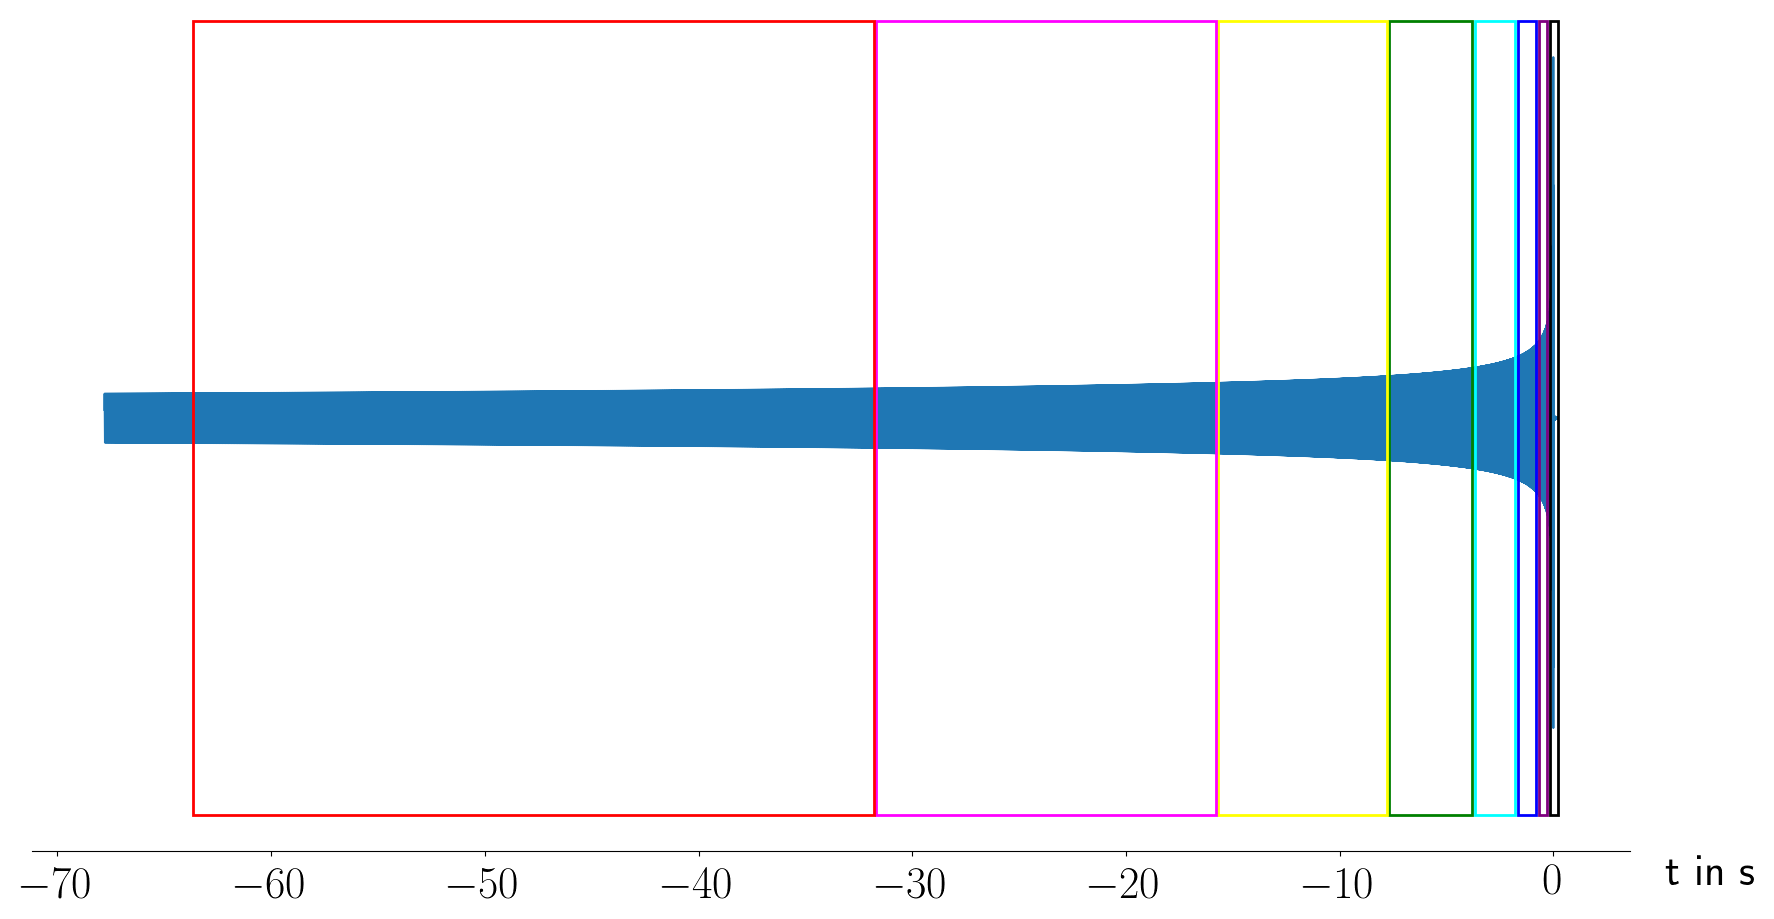
\includegraphics[width=\textwidth]{multirate_filtering_crop.png}
\caption[Multi-rate sampling]{The plot shows how each \gls{bns} signal is sampled at multiple rates. Only the last \SI{68}{\s} of the entire waveform are shown. Each sample rate and interval has its own color attributed. Specifically they are given by: black=(\SI{0.5}{\s}, \SI{4096}{\hertz}), purple=(\SI{0.5}{\s}, \SI{4096}{\hertz}), blue=(\SI{1}{\s}, \SI{2048}{\hertz}), cyan=(\SI{2}{\s}, \SI{4096}{\hertz}), green=(\SI{4}{\s}, \SI{1024}{\hertz}), yellow=(\SI{8}{\s}, \SI{512}{\hertz}), magenta=(\SI{16}{\s}, \SI{256}{\hertz}) and red=(\SI{32}{\s}, \SI{64}{\hertz}), where each tuple gives (segment duration, sample rate).}\label{fig:multirate_sampling}
\end{figure}
\medskip\\
A common drawback of training deep \gls{nns} is the need for large training sets. Luckily we are in a position where we can simulate our training samples and thus can generate an arbitrary amount. To do so we use the PyCBC software package \cite{pycbc}. The final training set contained $56250$ different signals and $161250$ different noise realizations. All of the noise samples were simulated using the analytic \gls{psd} \verb|aLIGOZeroDetHighPower| provided by PyCBC. Therefore all results obtained using this data only hold for stationary gaussian noise. All waveforms were generated using the approximant ''TaylorF2'', as implemented by PyCBC. \textcolor{red}{(Should this be Lal?)} Out of the 17 parameters that could have been varied, we fixed the spins to $0$ and neglected tidal effects for simplicity. Furthermore the coalescence time $t_\text{coal}$ is set to $0$ as well. The remaining $8$ parameters were chosen to represent a realistic distribution in order to estimate the potential of our approach in a real search. As such, both component masses $m_1$ and $m_2$ are uniformly distributed in the range \SIrange{1.2}{1.6}{M_\odot}. Specifically we do not explicitly require $m_1\geq m_2$ when generating the waveform. The coalescence phase $\Phi_0$  and the polarization angle $\psi$ are uniformly distributed on the interval $\left[0, 2\pi\right]$ and the inclination $\iota$ is distributed like $\arccos\lr{\text{uniform}\lr{-1, 1}}$. Finally the sky-position is isotropic, i.e. $\theta$ is distributed like $\arccos\lr{\text{uniform}\lr{-1, 1}}$ and $\varphi$ uniform in $\left[-\pi, \pi\right]$.\\
The luminsoity distance $r$ is chosen indirectly by fixing the \gls{snr} to some value. This is valid, as the \gls{snr} scales inversely with the distance. \textcolor{red}{(Is this true, or is for instance $SNR\approx 1/r^2$?))} In this work, the \gls{snr} is uniformly distributed on the interval $\left[8,15\right]$. One has to avoid one major pitfall when fixing or calculating the \gls{snr} and comparing it to other results. If one compares the \gls{snr} of two signals with the same parameters, the value will depend on the length of the segment used. According to \textcolor{red}{Reference to matched filtering section}, cutting off the waveform early might result in a lower or at least inaccurate value of the \gls{snr}. We therefore specify very precisely how we calculated the \gls{snr}. The waveforms are generated with a lower frequency cutoff of \SI{20}{\hertz}, which results in waveforms, with a duration of about \SI{500}{\s}. Afterwards the waveforms are projected onto the two detectors Livingston and Hanford and cropped in such a way, that they span \SI{96}{\s} and the shutoff lies within the last second. We vary the exact position of the highest amplitude between \SIrange{0.25}{0.75}{\s} from the end of the data stream and choose the signal that arrives at the latest point in time as reference. Only after the waveforms are cropped, we calculate the \gls{snr} of the pure signal (while assuming the \gls{psd} of the detector) using the waveform itself as a template. Since we are using multiple detectors, the \gls{snr} $\rho_i$ is calculated for each detector. The total \gls{snr} in the absence of noise is given by
\begin{equation}
\rho_\text{total} = \sqrt{\sum_i\rho_i^2}.
\end{equation}
Each waveform is than rescaled by multiplying with the factor $\text{\gls{snr}} / \rho_\text{total}$, where \gls{snr} is the target value. Each noise sample is labeled with \gls{snr} $4$ by convention. This value can in principle be picked freely but we chose it to resemble the average output of a matched filter search on pure noise. As a last step, before re-sampling the data as described above, the samples are whitened. To do so, we divide each of them by the amplitude spectral density given by $\sqrt{\text{\gls{psd}}}$. The \gls{psd} again is given by the analytic version \verb|aLIGOZeroDetHighPower| provided by PyCBC. Ideally one would use an estimate of the \gls{psd} to whiten the data. This is, however, not possible in our case, as we are storing signals and noise separately and only add them together at run time. Estimating the \gls{psd} would have the advantage of being more robust in a real search, as it would counteract drifts in the \gls{psd}.\\
The reason for storing noise and signals separately are resource constraints. To cover the entire parameter-space densely enough and avoid overfitting, a large number of samples is necessary. Initially we generated and stored the sum of signal and noise, instead of storing each category separately. This has multiple disadvantages, but also one key advantage; we can use the pure signal as a filter for the matched filtering \textcolor{red}{(Insert equation number here)}, thus  giving us an upper limit on the quality of the \gls{snr} a matched filter search could return. In that sense, we could monitor the performance and compare it to matched filtering directly during training. The disadvantages however at some point outweighed this advantage. The core one being the restricted number of samples. A file containing $500,000$ samples has a of \SI{\sim 200}{\giga\byte}. To train the networks on the data, we completely load it into system memory and need some overhead for formatting. To reduce these costs, we decided to split the signal- and noise-samples and only at runtime add together one instance of each category on the first layer of the network. The second advantage of this approach is less obvious. It enables us to easily feed the network the same signal submerged in multiple different noise realizations, which resulted in performance improvements for tasks similar to ours (Christoph Dreißigacker, personal communication, June 2019).\\
The split between training and validation set is treated with great care, assuring that not a single noise or signal sample from the training set is used during validation. Therefore the reported loss and accuracy values are representative of a real search. Though they are not the final statistic we report, they are tightly linked to those and give clues about the network and its efficiency.\\
The data used for training and validating the final network contained $75,000$ different \gls{gw}-signals and $215,000$ noise realizations\footnote{The numbers stated above were the number of samples in the training set. Here we are stating the numbers for the training and validation set combined, as they are stored in the same file. The numbers for the training set are a results of the split described below.}. We than generate a set number of unique index pairs $(s_i, n_i)$, where $s_i$ corresponds to a signal and $n_i$ to a noise sample. For the training set these indices may be selected from $s_i\in\left[0, 3/4s_t\right)$ and $n_i\in\left[0, 3/4n_t\right)$, where $s_t$ and $n_t$ are the total number of signals and noise samples respectively. If $3/4s_t\notin\mathcal{N}$ or $3/4n_t\notin\mathcal{N}$, the upper index is rounded to the nearest natural number. The total number of pairs generated is equal to the number of usable noise samples $3/4 n_t$. These index pairs represent all samples of the training/validation set that contain a \gls{gw}. In order to also supply pure noise samples to the learning algorithm, all noise realizations are also used during training. This is achieved by appending all index pairs $\lr{-1, 0}, \lr{-1, 1}, \dotsc, \lr{-1, 3/4n_t}$ to the list of index pairs generated before. Afterwards this list is shuffled. The \gls{nn} finally is fed with these $2\cdot 3/4 n_t$ samples through a function\footnote{Keras calls this function a generator.} that interprets the indices and reshapes the data. Overall the training set therefore consists of $322,500$ samples with a $1:1$-split between noise and signals. The validation set does have a $3:1$ split in favor of signals and contains the remaining $n_t / 4$ noise samples. Therefore, the validation set consists of $215,000$ samples.\\
The shape of the data depends on the network in use. Our final network expects a list of $16$ arrays, as we have $8$ different sample rates and a signal and noise input for each of them. The arrays are of shape $\lr{\text{mini-batch size, 2048, 2}}$. The last axis is the number of detectors used, whereas the second axis is the number of samples in the time series strain data.\medskip\\
Above we have only discussed the training and validation set in detail. The final results, however, are evaluated on the testing set. To eliminate most possible error sources, the testing set is generated completely independently from training and validation set, sharing only the distribution of parameters as discussed above. The testing set, furthermore, does not consist of individual samples, where each sample either contains a \gls{gw} aligned correctly or not, but is a set of continuous time series data. These large chunks are then handed to a generator function that chops each time series into overlapping blocks, i.e. sliding a window across the data. Each of these windows has a length of \SI{96}{\s}. The resulting chunk is whitened by dividing out the amplitude spectral density associated to the analytic \gls{psd} \verb|aLIGOZeroDetHighPower| and re-sampled to match the criteria of the network input. The window is than shifted by \SI{0.25}{\s} and the process repeated. The temporal resolution of \SI{0.25}{\s} was chosen because the waveforms are shifted around in the training set by \SI{\pm 0.25}{\s}. With the step chosen this way, we are guaranteed to have the maximum amplitude of the signal in the sensitive window of the network at some point. The result of sliding the network across the input data in the way described results in a \gls{snr} and p-score time series with time resolution \SI{0.25}{\s}. From these triggers can be generated by choosing some threshold based on the findings on the validation set.\\
The testing data was generated by Dr. Alexander Harvey Nitz using PyCBC but utilizing different functions.

\subsection{Network Metrics}\label{sec:network_metrics}
%\textcolor{blue}{Describe which metrics we use, why and how they are calculated.}\\
This section describes the different metrics we use to evaluate the performance of different networks. Not all of them were used throughout the entire time of testing architectures. For the final results we will only quote sensitivities at a given false alarm rate, which were also used to optimize the final networks. Early versions, however, were adjusted to optimize the variance and accuracy of the given predictions.\\
For the following it is important to note that we train all networks for two different output values. The first one is trained to estimate the \gls{snr} of a signal, the second one is trained to give the binary decision of whether or not a \gls{gw} signal is present. We will refer to these outputs by \gls{snr} and p-score respectively.

\subsubsection{Variance and Mean Squared Error}
The two metrics used to judge the performance of networks early on in the design process were the variance of the data and the \gls{mse} compared to the target value. Both of them were only applied to the \gls{snr} output. The reason for using these two was the simplicity of implementation and the fact that \gls{mse} is used as the loss function to optimize the network. As metric, the \gls{mse} gives an estimate of the average error for a prediction and thus is an estimator for the quality of predictions. The variance is an estimate of how far the recovered values spread and is hence a measure for the reliability of the prediction. The assumption was that these two metrics are strongly correlated with the sensitivity, which is the metric we want to report in the end.\\
Calculating the metrics is rather simple. We define the label values of our data by $y_\text{label}$ and the predictions by $y_\text{pred}$. If $y_\text{label}$ and $y_\text{pred}$ contain $n$ samples, the \gls{mse} is defined by
\begin{equation}
\text{\gls{mse}}=\frac{1}{n}\sum_{i=1}^n\lr{y_{\text{pred},i} - y_{\text{label},i}}^2.
\end{equation}
The variance is given by
\begin{equation}
\text{Variance}=\frac{1}{n}\sum_{i=1}^n\lr{y_{\text{pred},i} - y_{\text{label},i} - \text{mean}\lr{y_{\text{pred}} - y_{\text{label}}}}^2,
\end{equation}
with
\begin{equation}
\text{mean}\lr{x}=\frac{1}{n}\sum_{i=1}^nx_i.
\end{equation}
We aim to minimize both these metrics.

\subsubsection{False Alarm Rate}\label{sec:false_alarm_rate}
The false alarm rate is a measure of significance for any reported value. If we recover some value of \gls{snr} for given data, we need to know how reliable this value is and how likely it is to originate from pure noise. The false alarm rate therefore gives the number of noise samples per month\footnote{We define a month as 30 days.} that produce a higher ranking statistic than a given threshold. To estimate this function we need to sample
\begin{equation}\label{def:false_alarm_rate}
f(x)=\text{number of noise samples estimated louder than }x\text{ per month}.
\end{equation}
As we have two different ranking statics with our two outputs \gls{snr} and p-score, we also need to calculate two different false alarm rates. We furthermore need to differentiate between the discrete training/validation set and the continuous testing set. We will start by describing the process of estimating the false alarm rates for the training/validation set and afterwards go into detail about the differences for the testing set.\medskip\\
To sample $f$, we use the prediction values $x_i$ of our network for either of the two ranking statistics on pure noise samples. Let $m$ be the number of noise samples we have in the set and denote any specific noise sample by $n_i$. To estimate $f_i\coloneqq f(x_i)$, we define
\begin{equation}
f_i'\coloneqq \left|\left\{ x_j>x_i | j\in\left[1,m\right]\right\}\right|.
\end{equation}
$f_i'$ is the number of noise samples $n_j$ that got assigned a ranking statistic $x_j$ larger than $x_i$. It can therefore be understood as a cumulative sum. To convert this number to samples per time, we need to know how much time the $m$ samples span. To do so, we observe that for each signal the waveform is allowed to move around in the noise background by \SI{\pm 0.25}{\s}. Therefore, when we evaluate a continuous time series, we need to shift the network across the data with a step-size of \SI{0.25}{\s}. With this information the observation time $m$ samples cover is $m\cdot\vphantom{0.25}$\SI{0.25}{\s}. Therefore, $\frac{f_i'}{m\cdot 0.25}$ is in units ''samples per second''. From this we find $f_i=\frac{f_i'}{m\cdot 0.25}\cdot2,592,000$\SI[per-mode=fraction]{}{\samples\per\month} as an estimate for $f$, where $2,592,000$ is the number of seconds per month.\medskip\\
For a continuous stretch of data the notion of a noise sample is not as strictly defined. If we shift the window across the data, it might at some point contain only parts of a waveform. To resolve this issue, we set a threshold for the ranking statistic. If for any position of the window this threshold is exceeded we take this as a signal candidate. We then shift the network across the entire data with a step size of \SI{0.25}{\s} and take note of every position where the threshold is exceeded. In a next step these positions in time are clustered as a signal usually exceeds the threshold for multiple successive window positions. We do so by requiring two signal candidates to be within \SI{1}{\s} of each other to belong to the same cluster. Each cluster of signal candidates is then reduced to a single point in time by choosing the time where the ranking statistic is maximal. The signal candidate is finally assumed to be a false positive, i.e. originate from noise, if there is no injection within a time span of \SI{\pm 3}{\s} of it. The injection times are the times in the data where the waveform of an injection shuts off.\\
The false positive rate for continuous data is therefore a function of the threshold and gives the number of false positives per month at threshold $x$. To convert the number of false positives to samples per month, we again divide by the observation time, which in this case is given by the duration of analyzed data, i.e. \SI{4927488}{\s}. Finally we multiply it by $2,592,000$ to get it in units samples per month. \textcolor{red}{Not 100\% satisfied with this section yet, see if it can be improved.}
%To explain how we estimate this function, we will talk only about \gls{snr}. The process for the p-score, however, is equivalent.\\
%The values for $x$ we can sample are the predictions of the network over all pure noise samples. We will denote the number of pure noise samples by $m$. Each of these noise samples $n_i$ is evaluated by the network and assigned a \gls{snr} value of $x_i$. To estimate $f_i\coloneqq f(x_i)$, we define $f_i'\coloneqq \left|\left\{ x_j > x_i | j\in \left[1, m\right]\right\}\right|$. $f_i'$ therefore is a number of samples. To convert it to samples per month, we calculate the observation time, i.e. the time the total number of samples $m$ corresponds to. To do so, we observe that for each signal the waveform is allowed to move around in the noise background by \SI{\pm 0.25}{\s}. Therefore, when we evaluate a continuous time series, we need to shift the network across the data with a step-size of \SI{0.25}{\s}. With this information the observation time $m$ samples cover is $m\cdot\vphantom{0.25}$\SI{0.25}{\s}. Therefore, $\frac{f_i'}{m\cdot 0.25}$ is in units ''samples per second''. From this we find $f_i=\frac{f_i'}{m\cdot 0.25}\cdot2,592,000$\SI[per-mode=fraction]{}{\samples\per\month} as an estimate for $f$. We usually plot these results in a semi-log-scale plot, as the false alarm rate drops exponentially when going to higher \gls{snr}s.

\subsubsection{Sensitivity}
The sensitivity is the metric we are mostly trying to optimize. It gives the ratio of detected signals over total signals. To claim a detection we need to set a threshold for the detection statistic. Choosing this value in turn fixes the false alarm rate. So we can only claim statistical significance of the sensitivity if it is quoted alongside the associated false alarm rate.\\
As for the false alarm rate, we evaluate the sensitivity for both outputs individually. There are also slight differences between calculating it for the discrete training/validation set and the continuous testing set. Finally we can compute a volume from the found and missed signals in which our analysis is sensitive enough to find \gls{gw}-sources. We give these volumes in terms of a radius of a corresponding sphere. We will again start off by describing the process for the training/validation set.\medskip\\
The first step to calculating the sensitivity is fixing a threshold above which the network is thought of to have found a signal. As the training/validation set usually contain comparatively few samples, the false alarm rate can't be resolved at high thresholds or in other words we are not able to sample low false alarm rates. For this reason we choose the maximum value of the detection statistic of any noise sample as threshold. This usually corresponds to a false alarm rate of $\mathcal{O}\lr{10^3}$\SI[per-mode=fraction]{}{\samples\per\month}.\\
We then bin the training samples that contain a signal by their injected \gls{snr} and compute the ratio of how many samples in a bin get marked as signal over the total number of samples in that bin. For the training/validation set we do not compute the sensitive volume, as that would add another layer of complication and isn't useful for optimizing the performance, as the sensitive volume scales with the sensitivity.\medskip\\
For the testing set we plot the sensitivity against the false alarm rate rather than plotting it against \gls{snr} at fixed false alarm rate. We choose to plot against false alarm rate in order to have results that are comparable to matched filter results.\\
To obtain the sensitivity we need to figure out which injections have been found by the network and which have been missed. Therefore, the network is shifted across the continuous test set with a step size of \SI{0.25}{\s}. This creates a time series of detection statistic values. We then apply a threshold to this time series and flag anything that exceeds it as possible detection. These possible detections are then clustered as explained in \autoref{sec:false_alarm_rate} and declared a true detection if an injection is within a time span of \SI{\pm 3}{\s}. This generates a list of found injections as well as a list of missed injections. We furthermore know the parameters of each injection and can therefore infer an estimate of the sensitive volume using the PyCBC function \verb|volume_montecarlo|.\\
Fixing the threshold to some value also fixes the false alarm rate. We can therefore plot the sensitive volume against false alarm rate.
%To explain the sensitivity, we will again only go into detail about how we do this in terms of \gls{snr}, as the process for the p-score is equivalent.\\
%The sensitivity is a measure of how large the percentage of samples in a certain \gls{snr} bin are that get assigned a value larger than some threshold. We choose this threshold as the largest value that was assigned to some noise sample in our validation set, as we want to keep false alarms as low as possible. Therefore the first thing we do is find this maximal value. In a second step we look at all samples from the validation set, that contain a signal. For each of these signals the \gls{snr} value was chosen when injecting it into noise. For this reason, we can bin the samples based on this known value. Therefore, the x-values are the \gls{snr} values. (This is also true when calculating the sensitivity from the p-score.)\\
%The corresponding y-value is the number of samples in a bin assigned a higher value than our threshold over the total number of samples in a bin. In the case that a bin is empty, we assign it the value 0.

\subsection{Evolution of the Architecture}\label{sec:evolution_of_architecture}
%\textcolor{blue}{Talk about the different things we tried, what didn't work and how we improved on them. (Improvement from convolution to inception, improvement from inception to collect-inception, improvement from inception to tcn-inception, improvement of tcn-collect-inception over collect-inception.)}\\
%\textcolor{red}{Talk about the different loss functions used for the two outputs. Also mention their loss weights and training algorithms? Talk about general points we found, i.e. using dropout makes loss a little less stable but improves performance even when a lot of samples are used. (compare (24.06.2019) and (25.06.2019 (1)), (19.06.2019) and (25.06.2019 (2))) Decreasing learning rate in Adam did not help (19.06.2019).}\\
This section gives an overview of the steps that were taken to arrive at the final architecture. It chronologically highlights the pivotal points along the way and showcases some ideas that did not work out.

\subsubsection{Convolutional Network}\label{sec:evolution_convolution}
To start out we decided to test how well an architecture that is known to work well for \gls{bbh} signals holds up when it is trained on \gls{bns} signals. We therefore used an adaptation of the convolutional architecture introduced in \cite{huerta_parameter_estimation}.\\
As we only wanted to test how well the network could adapt to the new and different challenge, we decided to start with signals that are easy to find with traditional methods. Therefore, the \gls{snr} was uniformly distributed between 10 and 50, with all other parameters fixed. The neutron stars were modeled with $m_1=m_2=$ \SI{1.4}{M_\odot}. The data modeled the output of the two detectors Hanford and Livingston, using simulated noise and the waveform approximant TaylorF2. It contained samples of signals and pure noise realizations with a split of $1/2$ between the two. This data was further used until \autoref{sec:tcn_denoiser}.\\
The neural network consisted of 3 stacked convolutional layers, doubling the number of filters with every layer. The kernel size on the other hand was kept fixed at 16. We also introduced batch normalization layers in between each convolutional layer and the corresponding ReLU activation, as doing so had shown slight improvements when testing the network with \gls{bbh} data. As suggested by the original work, a maximum pooling layer was used after every convolution stack. Since the input data to our network is sampled at multiple rates, this network has 14 input channels instead of the 1 used in \cite{huerta_parameter_estimation}. (7 input channels per detector, where each of the 7 channels corresponds to a single sample rate) We also introduce a second output to the network and therefore use the output of the final convolutional stack as input for two different stacks of dense layers. The first reduced the number of neurons down to a single one, which is has the \gls{snr} as training goal, the second one condenses the output down to 2 values, which correspond to a binary decision. We will refer to these two outputs by the \gls{snr} output and the p-score output respectively. The two outputs use different loss functions to optimize the network. The \gls{snr} output is trained to match the injected \gls{snr} using a \gls{mse} whereas the p-score output gives two numbers that add up to 1. The first of these two numbers is trained to be 1 if the data contains a \gls{gw} and to be 0 if it is a noise sample. For this output we use a categorical crossentropy as loss. The total loss of the network is a weighted sum of these two outputs. We apply a weight of 1 to the \gls{snr} output and a weight of 0.5 to the p-score output, emphasizing the importance of recovering the \gls{snr}.\\
To rate the performance of a network we used only the \gls{mse} and variance of the \gls{snr} output and the false positive ratio of the p-score output with a threshold of 0.5. From these the sensitivity and false alarm rate can be eyeballed however. We will therefore also include crude estimates of these statistics here to put the performance of these networks into context of later improvements.\\
With a \gls{mse} of $\sim 6.5$, the network was able to recover the \gls{snr} rather well. The variance was on the same scale, also evaluating to $\sim 6.5$. The spread in recovered values is mostly down to the large \gls{snr} range attributed to pure noise samples, reaching from 0 up to 20. Using \gls{snr} 20 as a threshold to claim detection, the sensitivity can be eyeballed to reach 100\% only above \gls{snr} $\sim 25$ and dropping close to 0\% below \gls{snr} $\sim 20$. Furthermore, evaluating the second output on 3000 signals from the validation set gives an accuracy of about 95\% and a false positive rate of about 6\%. These numbers don't sound terrible but are in context. First of all, we try to optimize our network for the \gls{snr}-range of 5-15. At these values the false positive rate seems to be a lot higher than the 6\% over the entire validation set. Secondly, a false positive rate of 6\% equates to a false alarm rate of about \SI[per-mode=fraction]{6e5}{\samples\per\month}\footnote{This crude calculation uses 0.5 as a threshold value. Therefore, one gets $6\times 10^5$ samples with the output being larger than 0.5 per month.}. Ideally the false alarm rate should not exceed 1 per 2 months above an \gls{snr} of about $8$, as that false alarm rate is the threshold used to alert astronomers \cite{pycbc_live}. A month for this work is defined to be \SI{30}{\days}.\\
From this we concluded that it is possible for a \gls{nn} to learn to classify \gls{bns} data but further improvements to the architecture are necessary to reach desirable sensitivities at acceptable false alarm rates.
%The first architecture we used was very close in nature to that of \cite{huerta_parameter_estimation}, halving, however, the number of filters in each convolutional layer and using batch normalization in between the convolution and its activation. Therefore, we used a network of 3 stacked convolutional layers, each followed by a batch normalization, ReLU activation \textcolor{red}{(Never introduced the ReLU activation)} and maximum pooling layer. The number of filters was doubled after each convolutional layer. Since the input data to our network is sampled at multiple rates, this network has 14 input channels instead of 2. (7 input channels per detector, where each of the 7 channels corresponds to a single sample rate)\\
%Though initially trained without pure noise samples and with only the \gls{snr} as training goal, we soon changed to use the data as mentioned in the beginning of this section. Furthermore, we added a second output. This second output gives a number between 0 and 1, where 1 corresponds to the network classifying the data as signal and 0 for classifying it as pure noise. If the output is neither 0 nor 1 one can use a threshold to determine if the output should correspond to a signal or pure noise. By default the threshold value is set to $0.5$. We will refer to the results this output gives as ''p-score'' throughout this work, even though it is not really a probability. As this second output tries to categorize the results into two different classes, it is inefficient to use mean squared error as a loss for this output. Instead we use a loss called categorical crossentropy, which is designed to optimize classification problems. As we are using two different losses now, the network will optimize the sum of the mean squared error from the \gls{snr}-output and the categorical crossentropy from the p-score output. This furthermore requires us to split the last layer into two.\\
%All of the following analysis is based purly on (13.02.2019) in \cite{network_wiki} and its limited information. Therefore, a lot of the statements below are only qualitative rather than quantitative.\\
%Due to the limited statistics calculated at the time, a lot of the statements below are solely qualitative rather than quantitative.\\
%The network was able to recover the \gls{snr} of signals rather well but has a large spread for the recovered \gls{snr} values of pure noise samples. The sensitivity can be eyeballed to reach 100\% only above \gls{snr} $\sim 25$ and dropping close to 0\% below \gls{snr} $\sim 20$. The latter is caused by the high \gls{snr} values assigned to certain noise samples, some reaching values of up to $\sim 20$. Furthermore, evaluating the second output on 3000 signals from the validation set gives an accuracy of about 95\% and a false positive rate of about 6\%. These numbers don't sound terrible but are in context. First of all, signals are expected to be in the \gls{snr}-range of 5-15 \textcolor{red}{[Citation]}. At these values the false positive rate seems to be a lot higher than the 6\% over the entire validation set. Secondly, a false positive rate of 6\% equates to a false alarm rate of about \SI[per-mode=fraction]{6e5}{\samples\per\month}\footnote{This crude calculation uses 0.5 as a threshold value. Therefore, one gets $6\times 10^5$ samples with the output being larger than 0.5 per month.}. Ideally the false alarm rate should not exceed 1 per 2 months above an \gls{snr} of about $8$, as that false alarm rate is the threshold used to alert astronomers \cite{pycbc_live}. A month for this work is defined to be \SI{30}{\days}.

\subsubsection{Inception Network}\label{sec:evolution_inception}
The first major improvement to the original architecture was the introduction of the inception module \cite{inception_module}. This new module had shown strong improvements for the image recognition challenge \gls{ilsvrc} in 2014, replacing traditional convolutional layers. As image recognition is one of the most active fields for the development of new \gls{nn} architectures, we decided to test if their findings are applicable to time series data as well.\\
We applied the same data and used the same output data as in \autoref{sec:evolution_convolution}.\\
The inception modules were a direct adaptation of the 2 dimensional variant presented in \cite{inception_module}. Details can be found in \autoref{sec:inception_module}. To get the best comparison of performance to the pure convolutional architecture of \autoref{sec:evolution_convolution}, we used basically the same architecture. The three convolutional layers of the old architecture were simply replaced by inception modules. The number of filters, however was kept constant and the kernel size was adjusted. The original work suggests to use kernel sizes of $(1,3,5)$ within the inception module. We found that using slightly larger kernel sizes $(4,8,16)$ improved our statistics significantly. Another adaptation to the architecture used in \autoref{sec:evolution_convolution} is the use of two further convolutional layers before the first inception module. These again improved performance and were inspired by \cite{inception_module}. Overall the network consisted of two convolution layers, followed by three inception modules and funneled down to the final outputs using two dense layers.\\
With these alterations to the architecture the \gls{mse} dropped to $\sim 4.5$ and the variance to $\sim 3.9$. These are significant improvements over \autoref{sec:evolution_convolution}. As reference, the goal was to reach values of \gls{mse} and variance around $2$ in order to use more difficult to detect data. Furthermore, the false positive rate dropped to $\sim 0.015\%$ which corresponds to a false alarm rate of only \SI[per-mode=fraction]{\sim 10e3}{\samples\per\month}. This is already pretty good for first tests. The sensitivity at this false alarm rate went up to 100\% around \gls{snr} 20 and only dropped to 0\% below \gls{snr} $\sim 12$. This improvement is down to the loudest false positive only being estimated to have \gls{snr} $\sim 15$.\\
Though this is still not an impressive performance, it is a considerable improvement over the simple convolutional approach and shows the potential inception architecture for time series data.\medskip\\
We also tried to evaluate the necessity of all the different sample rates for the network, as it can be beneficial in multiple ways to reduce the number of input samples. We therefore trained the same network using different sample rates. Adding sample rates one by one, the first network was trained using only the \SI{2048}{\hertz} data, the second used both the \SI{2048}{\hertz} and the \SI{1024}{\hertz} data and so on. We also tried to use only the three sample rates\SI{2048}{\hertz}, \SI{512}{\hertz} and \SI{128}{\hertz}, as we expected them to contain the main frequencies. We found however that each sample rate, except for \SI{64}{\hertz}, improved the performance of the network. Using only the three sample rates that we expected to work best, however, was also very close in performance to using all sample rates in this test. The \SI{64}{\hertz} sample rate on the contrary seemed to hurt performance.\\
We also tested different depths of inception architectures and found that shallower networks usually perform a bit better than deeper ones. This probably points to a vanishing gradient problem. We however did not verify this hypothesis.
\begin{comment}
From this point the first major iteration was the introduction of inception modules \cite{inception_module}. They replaced the simple convolutional layers of the architecture used previously.
%(see 15.02.2019 and 03.04.2019 in \cite{network_wiki})
 Furthermore, guided by \cite{inception_module}, the inception modules were preceeded by 2 convolutional layers. The implementation of the inception module was as a first step a direct adaptation of the original work \cite{inception_module}. It used kernel sizes of $\lr{1,3,5}$. With these kernel sizes, results did not improve but rather got worse. Increasing the filter sizes to $\lr{4,8,16}$, however, proved to be a useful change. The performance in mean squared error, variance and false positive rate improved significantly, with the false positive rate reaching $\sim 0.015\%$. By eye, the sensitivity also made an improvement as the loudest false positive was estimated to have \gls{snr} $\sim 15$. With this, the sensitive went up to 100\% around \gls{snr} 20 and only dropped to 0\% below \gls{snr} $\sim 12$. Though this is still not an impressive performance, it is a considerable improvement over the simple convolutional approach.\medskip\\
Having found the new inception architecture, we conducted a test to figure out which of the 7 sample rates benefit the network the most.
% To view the full results see 04.04.2019 and 05.04.2019 of \cite{network_wiki}.
 We found, that each sample rate, except for the \SI{64}{\hertz} one, benefits the results. Using only the sample rates (\SI{2048}{\hertz}, \SI{512}{\hertz}, \SI{128}{\hertz}) gave comparable results to using the channels (\SI{2048}{\hertz}, \SI{1024}{\hertz}, \SI{512}{\hertz}, \SI{256}{\hertz}, \SI{128}{\hertz}). Furthermore, shallower networks seemed to yield similar or improved performance, when compared to deeper ones. Shallower and deeper in this case refers to the number of stacked inception modules.
\end{comment} 
 
\subsubsection{Collect-Inception Network}\label{sec:evolution_collect_inception}
As we are using multi-rate sampling for our input data, we wanted to test if it would be beneficial to the performance to have the network analyze each sample rate separately and and only combine the results in the end. Considering the findings of \autoref{sec:evolution_inception} only the three sample rates \SI{2048}{\hertz}, \SI{512}{\hertz} and \SI{128}{\hertz} were used in the beginning. The data was split for the three inputs, each containing the data for 2 detectors.\\
The architecture consisted of three inception networks side by side, the results of which were concatenated and put through some final dense layers. Each inception network consisted of multiple stacked inception modules. In the beginning these did not all have the same depth, but we empirically found the network would perform best if each stack contained the same number of inception layers. With further testing we found that shallower networks for each sample rate and a small inception network after concatenating the stacks improved results even further. The final iteration of improvement found that using all sample rates improved the performance of this architecture even further. Therefore the final network, for which we will give the metrics below, consisted of 7 parallel stacks of three inception modules each. The results of these stacks are then concatenated and used as input for two further inception modules. Their output is finally passed to two further dense layers for each output.\\
This architecture managed to bring down the \gls{mse} to $\sim 2.5$ and the variance to $\sim 2.4$. With this we had just about reached our goals for the simple data. The false positive rate, however, was higher by about 20 times for this network when compared to the architecture presented in \autoref{sec:evolution_inception}. Furthermore, the false alarm rate for the loudest noise sample is about twice that of the previous network. The sensitivity at this higher false alarm rate on the other hand also improved slightly. It didn't drop to 0\% even at \gls{snr} 10 and reaching 100\% at \gls{snr} $\sim 18$. However, we did not consider the latter metrics at the time of testing the networks and only looked at \gls{mse} and variance. For this reason, the new collect-inception architecture was the clear choice to move on. Later findings will back this conclusion up, even though we should not have drawn it for this architecture.\\
Having a worse estimate of the false alarm rate is due to the a lower number of noise samples used in the validation set. At the time we were testing many different architectures and data setups. For that reason not all validation sets were similar enough to draw good conclusions. For others who try to compare different architectures we therefore want to point out that using a single validation set for all networks is vital for the efficient improvement of architectures.\smallskip\\%\textcolor{red}{Mention that we used less data in the validation set (or overall), which leads to worse upper bounds on the false alarm rate. To have comparable results, the same validation set or at least the same number of noise samples should be used. Why did we use fewer samples? Computational cost?}\medskip\\
As we had reached out goal of \gls{mse} and variance for the easy data with this network we changed to use more difficult data from here on out. For details see the following section. We will refer to a network consisting of multiple parallel stacks of inception layers as ''collect-inception network'' from here on out.
\begin{comment}
Having found that using only the sample rates (\SI{2048}{\hertz}, \SI{512}{\hertz}, \SI{128}{\hertz}) is at least a good approximation to using all sample rates, we tested a new architecture. Previously all sample rates were fed to the network in terms of channels of the same convolutional layer. The new architecture assigned a stack of inception modules for each sample rate. This way the channels only represent the different detectors. The result of each stack are than concatenated and fed to some final layers. In the beginning the stacks for different sample rates had different depth. We found however that the network functioned best when each stack had the same depth. Furthermore, results improved when the stacks were not too deep. We settled on an architecture that had a depth of 3 inception modules in each stack, deployed another 2 inception modules after concatenation and condensed them down to the ouput size by the use of 2 dense layers per output.\\
As a last step, we tested the performance of using the three sample rates mentioned above against using all sample rates. Here using all sample rates improved the results significantly. Therefore, the performance quoted below is derived from the network using all sample rates.
% For the full history on the evolution and architecture of these kinds of network see (12.04.2019 (2)) through (17.04.2019) in \cite{network_wiki}.
 From here on out, we will call a network that uses individual stacks of layers for each sample rate a collection network. Therefore we call the kind of network described above a ''collect-inception network''.\\
The final iteration of this architecture broke the previous records of mean squared error and variance against the label values. With a false positive rate of $\sim 0.3\%$, it did perform worse than the previous record holder. This was, however, not the metric we judged the performance by at that point in time. Therefore, this network was thought of as the best one. By eye, one can also estimate that the sensitivity didn't drop to 0\% even at \gls{snr} 10 and reaching 100\% at \gls{snr} $\sim 18$. In this aspect the network improved.\medskip\\
The performance of this newest iteration of the network was good enough for us to move on to a more difficult data set. For this one we only changed the \gls{snr} range. Instead of varying it between 10 and 50, we went down to varying it between 8 and 15. Furthermore, we introduced sensitivity and false alarm rate as new metrics to gauge performance. We calculate both of these statistics for each of the two outputs and in the following way.\\
\end{comment}

\subsubsection{Temporal Convolutional Denoiser}\label{sec:tcn_denoiser}
After the success of the collect-inception network introduced in \autoref{sec:evolution_collect_inception} we were inspired by \cite{tcn_idea} to try a new kind of network, called temporal convolutional network (\gls{tcn}). Their results suggested that a stack of dilated convolutional layers outperforms normal stacked convolutional layers when classifying data containing \gls{gw} signals. Their idea was backed up by findings of \cite{tcn_paper}, who showed that \gls{tcn} are better suited for sequence data than other architectures.\\
Since the collect-inception network achieved our metric goals for the simple data, we started to use more difficult data from this point on. We still kept all parameters but the \gls{snr} fixed, but varied the latter one between $8$ and $15$ instead. We furthermore feed the network noise and signals separately now and add them together on the first layer of the network. Doing so has many advantages. First of all it gives us more effective samples (see \autoref{sec:data_generating_process} for details). The second reason comes from the properties of the \gls{tcn}. As we are training for \gls{snr} and p-score, one immediate problem of a pure \gls{tcn} would be the output shape. This kind of network was originally designed to generate and alter sequence data and thus returns a tensor of the same length per channel as its input. This would be great, if we could generate a \gls{snr} time series for all inputs as training goal. We would then simply get an estimate of the \gls{snr} time series as output from our network (compare \cite{cnn_magiacal_bullet}). It is, however, not trivial to do so and for our purposes impractical\footnote{Defining a \gls{snr} time series for data that is sampled at multiple rates is the technical difficulty. The impracticality does only come in, when we store noise and signals separately, as we would need to generate the \gls{snr} time series on the fly, which is computationally expensive.}. The first intuitive solution to the problem of reshaping would simply be to use dense layers to scale down the output to the desired dimensions. We did try this approach but had no success. Instead, inspired by \cite{dnn_denoising}, we used the \gls{tcn} as a denoising stage in front of every input of the collect-inception network. To train the \gls{tcn} to be a denoiser, we need the pure waveform as training goal. It is therefore convenient to store waveform and noise separated.\\
The \gls{tcn} consisted of 12 stacked dilated convolutional layers, where the dilation factor was set to $2^i$ with $i$ being the number of convolutional layers that came before. The number of convolutional layers was chosen such that the receptive field of the network spanned the entire 4096 input samples. For details of the exact implementation of the \gls{tcn} see \autoref{sec:tcn}. We used one \gls{tcn} in front of every input to a collect-inception network. To train the \gls{tcn}s to be denoisers, each of them was trained to recover the pure waveform from noisy data. Therefore an auxiliary output was added after every \gls{tcn} that got the pure input waveform as training goal. The used loss was \gls{mse} and assigned a weight of 1. Its output is then added back onto the sum of noise and signal and collectively used as input for a collect-inception network with an architecture that was discussed in \autoref{sec:evolution_collect_inception}. The idea behind adding the \gls{tcn}-output back onto the input was to amplify signals, whilst not throwing away information, if the \gls{tcn} was not able to recover a signal.\\
This new architecture and data was also the point in time where we started to use the false alarm rate and sensitivity at that false alarm rate as metrics to judge the performance. The false alarm rate can be estimated to be \SI[per-mode=fraction]{\sim 250}{\samples\per\month} at \gls{snr} $\sim 9.5$. Fixing the false alarm rate to this value allows us to calculate the sensitivity, which outperformed any previous architecture. It did not drop below 20\% in any \gls{snr} bin even down to \gls{snr} 8. Furthermore the sensitivity stayed above 80\% for \gls{snr}s $\leq 12$. All these values are quoted at lower false alarm rates than those achieved in \autoref{sec:evolution_inception} and \autoref{sec:evolution_collect_inception}. To still compare the \gls{mse} and variance to earlier architectures, the \gls{mse} reached a value of $2.7$ and the variance $2.3$. These are slightly worse values than recorded before but achieved using more difficult data. We also tested to use the architecture presented in \autoref{sec:evolution_collect_inception} on this more difficult data set and found that even though the \gls{mse} and variance at $2.6$ and $1.9$ are lower, the sensitivity is worse. This is especially true for the lower \gls{snr} bins. However, the false alarm rate used to determine the sensitivity again was different to that used to estimate the sensitivity of the collect-inception network using a \gls{tcn} as a denoiser. For the pure collect-inception network the false alarm rate was set to be \SI{\sim 100}{\samples\per\month}. We did, however, not consider this offset in false alarm rate at the time. A collect-inception network using a \gls{tcn} as a denoiser will be called a \gls{tcn}-collect-inception network or short \gls{tcin} from here on out.\\
Even though the \gls{tcin} architecture was considered to work a lot better than previous attempts it had the major downside of complexity. Using an individual \gls{tcn} for each sample rate and following it up with a collect-inception network required about \SI{30}{\giga\byte} of memory with a mini-batch size of only 24 samples. The only graphics card that can has enough video memory is the NVIDIA GV100. The availability of this hardware is very limited and thus does not allow for rapid development. A smaller alternative would therefore be highly beneficial.\\
We also conducted a test, trying to determine if the \gls{tcn} is able to reconstruct the original waveform from a noisy time series. These tests showed that it is not consistently able to do so. Using mean average percentage error as a loss function and setting the noise free signal as the training goal for a pure \gls{tcn}, the loss did not fall below $70,000$. Trying to train the \gls{tcin} without the use of an auxiliary loss function, however, proved to deteriorate performance. Therefore, other \gls{tcin}s use the auxiliary outputs as well.
\begin{comment}
For the first few iterations the sensitivity is calculated slightly wrong, as the p-score output was used in the case of the \gls{snr}-sensitivity to judge whether or not we were looking at a false positive. In that sense a false positive was a noise sample, where the p-score was greater than $0.5$, thus impacting the threshold used. As the outputs for \gls{snr} and p-score tend to be highly correlated however, the differences was not significant and most of the values are close to the real sensitivities. The false alarm rates were also not calculated correctly for the first few runs, as they were always scaled by the same factor, regardless of how many samples the validation set actually contained. We try to not report these bad false alarm rates.\medskip\\
After using the previously best known architecture and taking a quick look at the sensitivity it was able to reach, we were inspired by \cite{tcn_idea} to try a new kind of network, called temporal convolutional network (\gls{tcn}). Their results suggested that a stack of dilated convolutional layers outperforms normal convolutional layers. Their idea was backed up by findings of \cite{tcn_paper}, who showed that \gls{tcn} are better suited for sequence data than other architectures. We could however not directly test their implementation as they did not reveal their entire architecture. \textcolor{red}{(I don't have access to the quoted paper in its present state, so maybe they did reveal it. Can I get access?)}\\
As we are training for \gls{snr} and p-score, one immediate problem of a pure \gls{tcn} would be the output shape. This kind of network was originally designed to generate and alter sequence data and thus returns a tensor of the same length per channel as its input had. This would be great, if we could generate a \gls{snr} time series for all inputs as training goal. We would then simply get an estimate of the \gls{snr} time series as output from our network (compare \cite{cnn_magiacal_bullet}). It is, however, not trivial to do so and for our purposes impractical\footnote{Defining a \gls{snr} time series for data that is sampled at multiple rates is the technical difficulty. The impracticality does only come in, when we store noise and signals separately, as we would need to generate the \gls{snr} time series on the fly, which is computationally expensive.}. The first intuitive solution to the problem of reshaping would simply be to use dense layers to scale down the output to the desired dimensions. We did try this approach
%rather late (see (25.07.2019 (1)) in \cite{network_wiki})
 but had no success. Instead, inspired by \cite{dnn_denoising}, we tried to use the \gls{tcn} as a denoising stage in front of every input stack of the collect-inception-network. To do so, we fed each input to a \gls{tcn} and added an auxiliary output afterwards. This output used a mean squared error loss to fit the pure waveform in the Livingston detector. The output of the \gls{tcn} is than added back onto the input and fed into a stack of 3 inception modules. The result of each such stack are finally concatenated and fed into dense layers. Each \gls{tcn} consisted of 12 dilated convolutional layers. The number of convolutional layers was chosen such that the receptive field of the \gls{tcn} covers the entire length of the input, i.e. 4096 samples. The idea behind adding the \gls{tcn}-output back onto the input was to amplify signals, whilst not throwing away information, if the \gls{tcn} was not able to recover a signal.\\
 % Details of this architecture and the results we found can be viewed at (03.06.2019) in \cite{network_wiki}. \textcolor{red}{(Insert image of general architecture)}\\
Using the \gls{tcn} as a denoiser required us to change the way the samples are fed to the network, as we needed the pure \gls{gw}-signal for the training goal. Thus, instead of feeding the network the sum of signal and noise, it receives the two parts separately and adds them together on the first layer. When evaluating real samples the network will be fed the sum of signal and noise instead. This is not a problem though, as one of the two inputs can simply receive zeros as input. This is a change to the data generation we decided to keep. For a detailed reasoning as to why we decided to keep that change see \autoref{sec:data_generating_process}.\\
The performance of this network exceeded those of any previous network by a considerable margin. Now judging by sensitivity rather than mean squared error or variance, it dropped below 80\% sensitivity only for \gls{snr}s smaller 12 and didn't considerably drop below 20\% at all. The sensitivity improved especially at low \gls{snr}s. Using $37,500$ noise samples the false alarm rate can be resolved up to about \gls{snr} 9, as that is the value of the loudest sample. Below \gls{snr} 9 the false alarm rate is rather high with a lowest value of about \SI[per-mode=fraction]{300}{\samples\per\month}. Using more noise samples would enable us to finer resolve the false alarm rate. As it is not feasible during development, to evaluate each individual network on a large set of data, we will only use the sensitivity to get a rough estimate of the performance and compare different algorithms in that regard. For the final network a large testing set will be used in order to more finely resolve the false alarm rate and to make stronger statements on the sensitivity.\\
From here on out we will refer to a network of the kind described in this part as \gls{tcn}-collect-inception network or \gls{tcin}. Though it improves almost all statistics we are using, when compared to a standard collect-inception network, it comes at a cost. This cost is the memory the network needs in order to be trained. In the form used for these results, it used \SI{30}{\giga\byte} of video memory on a NVIDIA GV100 while already reducing the mini-batch size to only 24. This graphics card is currently the only one that has enough memory to support such an architecture. The availability of this hardware is very limited and thus does not allow for rapid development. A smaller alternative would therefore be beneficial.\\
We also conducted a test, trying to determine if the \gls{tcn} is able to reconstruct the original waveform from a noisy time series. These tests showed that it is not consistently able to do so. Using mean average percentage error as a loss function and setting the noise free signal as the training goal for a pure \gls{tcn}, the loss did not fall below $70,000$. Trying to train the \gls{tcin} without the use of an auxiliary loss function, however, proved to deteriorate performance.
% (see (24.07.2019 (2) in \cite{network_wiki} for details)
 Therefore, other \gls{tcin}s use the auxiliary outputs as well.
 \end{comment}
 
\subsubsection{Evolution using Bad Data}\label{sec:evolution_bad_data}
After the success of \gls{tcin}s, we searched for simpler architectures to reduce memory constrains. For that reason we tried using an old record holder, a simple inception network that was very memory efficient. To improve its performance, residual connections were added to every inception layer where it was possible to do so without needing to use dimensional reduction layers. This choice was motivated by a conversation with Christoph Dreißigacker and the results of \cite{residual_connections_invention}. The residual connections are meant to help the network learn as it is more easily able to recover the identity mapping between the input of an inception module and its output.
% (see (26.06.2019 (1)) and (27.06.2019 (1)) in \cite{network_wiki})
 The total network consisted of 8 stacked inception modules with one intermediate pooling layer and 6 residual connections. Networks using mainly inception modules and combining them with residual connections will be called inception-res networks from here on out. The inception modules were preceded by two convolutional layers. The different sample rates were fed to the network as different channels of the same input layer. It also only used the three sample rates (\SI{2048}{\hertz}, \SI{512}{\hertz}, \SI{128}{\hertz}). By accident, the kernel sizes in the inception modules were set to $(1,2,3)$. This did, however, prove to be beneficial to the network.\\
The results this network produced were incredible and outperformed anything we had seen so far. Sensitivities stayed close to or above 60\% for all \gls{snr} bins and the loudest noise sample was estimated at an \gls{snr} of $\sim 7.8$. One thing that seemed strange though, was the plot of recovered \gls{snr}s against the label values. For some specific \gls{snr} values, the predictions were scattered but lower by a significant margin. This can be seen as streaks when plotting the recovered against the label values, as done in \autoref{fig:streak_plot}.\smallskip\\
\begin{figure}
\centering
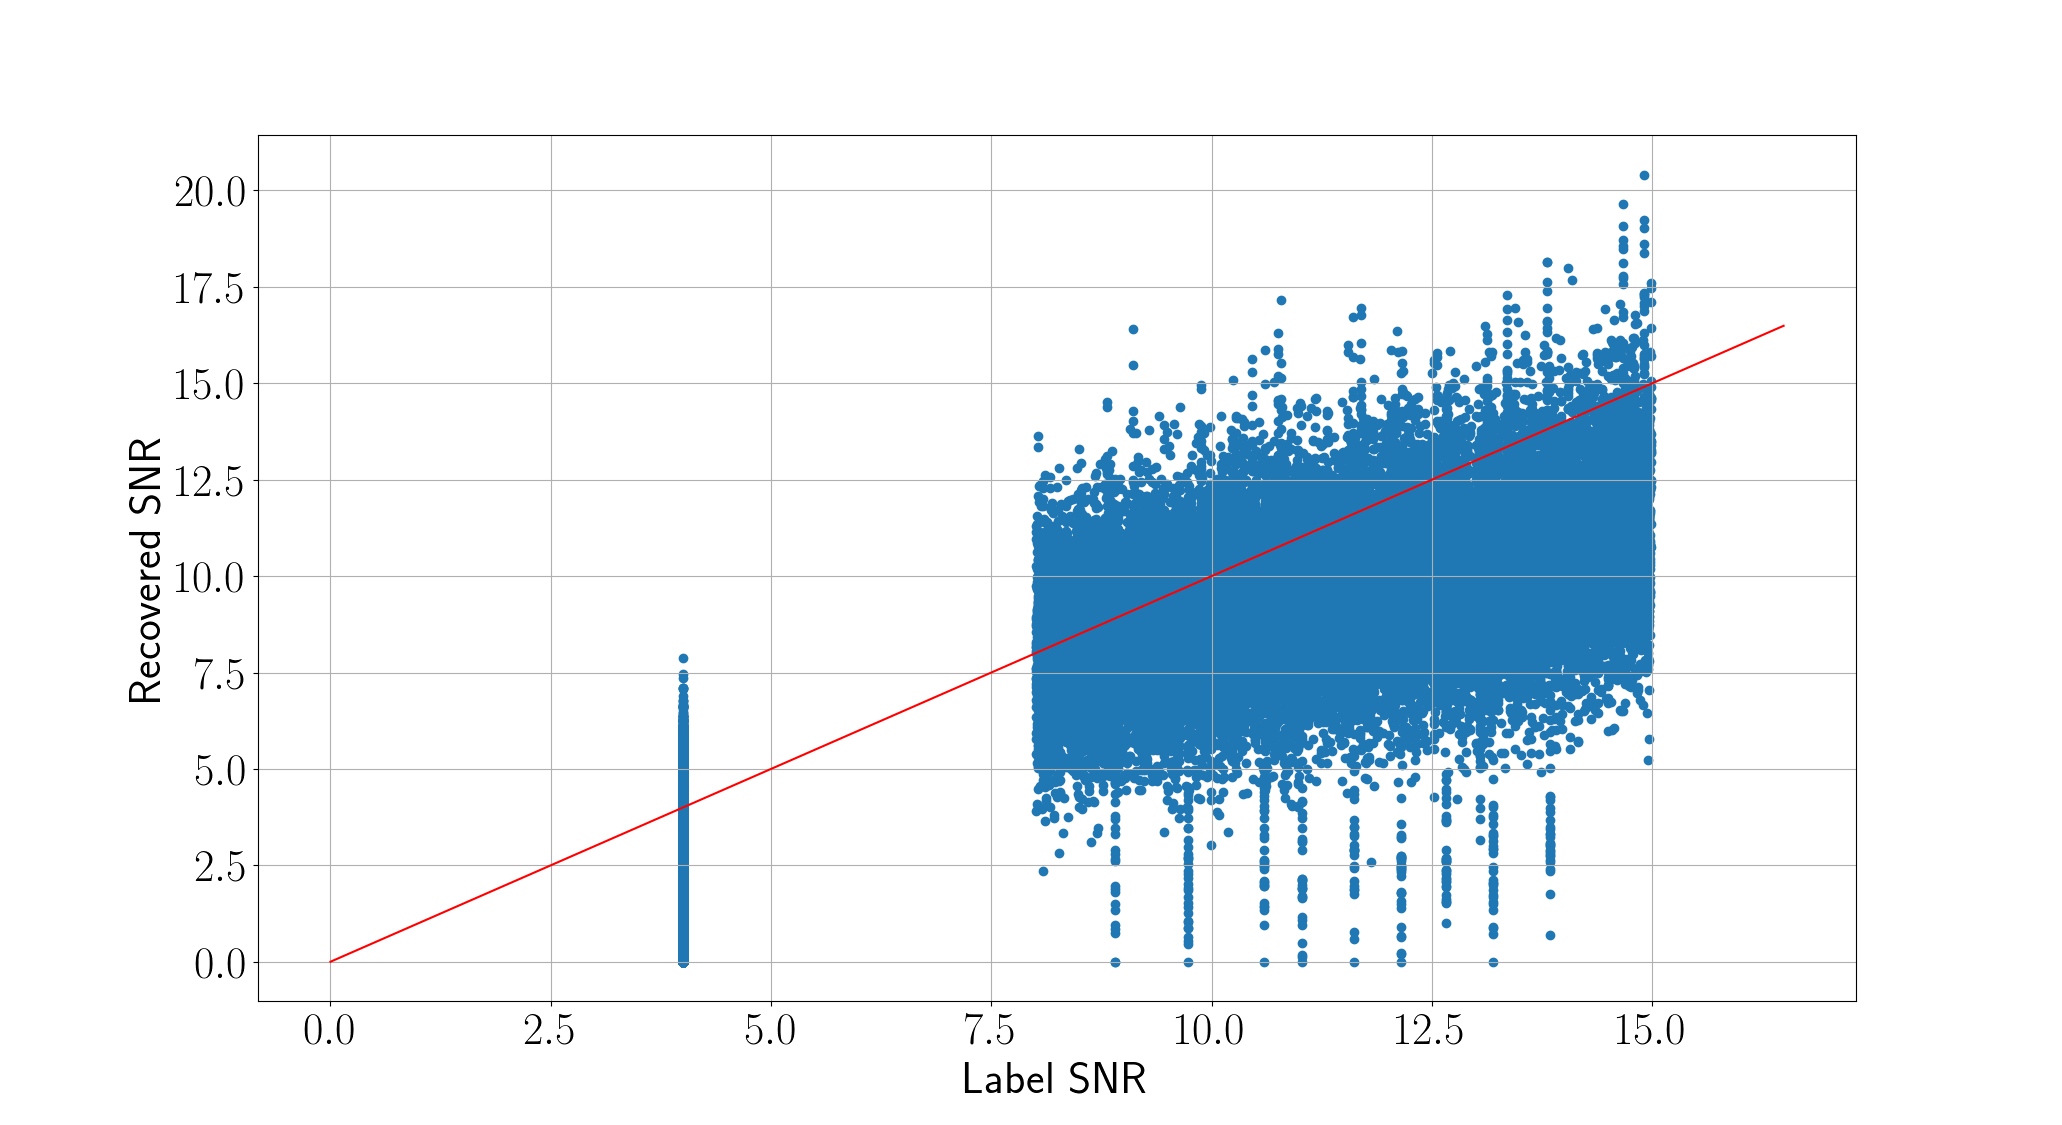
\includegraphics[width=0.75\textwidth]{streak_plot.png}
\caption[Plot of recovered values showcasing an error]{Shown are the recovered \gls{snr} values on the y-axis and the label values on the x-axis. Each \gls{snr} label has multiple y-values assigned to it, as the same waveform is submerged in multiple different noise realizations. The red line indicates where the dots should lie if the network recovered them without error. The dots roughly follow this line with the exception of a few streaks going down to 0. These are the waveforms that resonate strongly with the signal that was mistakenly added to every pure noise sample. Later iterations of the architecture reduced the number of streaks down to a single one.}\label{fig:streak_plot}
\end{figure}
The observed behavior and the incredible performance was due to a bug in how the network was fed with data. The generator combines a pure waveform with one noise realization to create a signal sample and is supposed to combine an array of zeros with a noise realization for a pure noise sample. A missing ''if''-statement led to the array of zeros always being replaced with the waveform that was the last in the list of available waveforms. Therefore, instead of pure noise, the network always saw noise plus one specific waveform. The same error with the exact same waveform was present in both the training and the validation set which made this error hard to catch. In fact the error was only discovered about two weeks after it first occurred. Finding the bug this late led to the optimization of the architecture for this flawed data. The best performing network had a sensitivity of more than 95\% over the entire \gls{snr} range for this flawed data, even once we used more difficult data, i.e. varying more parameters than just the \gls{snr}.\\
Though this mistake might at first seem like a waste of time, it actually helped in two aspects. Firstly, it showed the possibility for a network to consistently recover a single sample from different noise realizations and being able to model it well enough. The hurdle for a general search isn't trivial from this point, as in an optimal case we would expect the network to generalize the structure of the waveforms it was trained on and interpolate a template bank, but it is a starting point. Secondly, the optimization led to architectures with improved performance over for instance the \gls{tcin}s, when evaluated on non-flawed data. For this reason, we will list a few of the notable improvement here.\smallskip\\
The first observation was that the mistake of using filter sizes $(1,2,3)$ was actually an improvement over using $(4,8,16)$, which was previously used and found to be beneficial.
% (see (27.06.2019 (2)) in \cite{network_wiki}).
 Another feature introduced was the reduced number of input samples. Before the different sample rates had some overlap in the time domain, i.e. the last second of the data was sampled by all 7 rates, the last 2 seconds were sampled by all but the highest sample rate and so on. As the higher sample rates also contain all the information the lower sample rates do, this overlap was thrown away. For a detailed description of how this non overlapping multi-rate sampling works see \autoref{sec:data_generating_process}. A study, testing the two different approaches to sampling the data and reducing the number of input samples by simply using less sample rates, showed that using all sample rates is beneficial, while cropping the overlapping part of the data has no considerable negative effect.\\
 % (see 02.07.2019 (2) and following in \cite{network_wiki})\\
With the performance these architectures suggested, we moved to more difficult data, altering not only the \gls{snr} but also component masses $m_1, m_2$, coalescence phase $\Phi_0$, sky-position $\theta, \varphi$ and inclination $\iota$. As expected, the performance decreased a bit using more difficult data. Trying to recover the old performance led to one of the final improvements to the architecture. Instead of using a single inception stack, we introduced an architecture that is a mixture of the collect-inception networks and the pure inception networks. It uses the same inputs as the collect-inception networks, but cascades down concatenating two stacks after two inception layers, reducing the initial 8 stacks to 4. These 4 stacks each are fed through two further inception layers before being concatenated again. This procedure is repeated a third time, which results in a single stack of inception layers which is than fed to dense layers, in order to get the outputs. See \autoref{fig:cascade_inception_res_net} for an overview of the architecture. We will still refer to networks with a similar structure as collect-inception-res networks.\\
It again improved results a by a little. The sensitivity now didn't drop below 97\% for any of the bins, with the loudest noise sample having an \gls{snr} $\sim 8$. This is the last and best performing iteration of the network we found before the bug in the generating process was discovered and fixed. It therefore is still one of the core structures of the final architecture.\smallskip\\
After the error in the data generator from \autoref{sec:evolution_bad_data} was caught, we tried to evaluate how large of an impact it made. We therefore tested the different architectures we had found to be working well for the flawed data on the corrected data, which still varied component masses, coalescence phase, sky position and inclination.\\
The inception-res network experienced a drop in sensitivity to below 20\% in the loudest \gls{snr} bin. The collect-inception-res network held up a bit better, with its sensitivity dropping only to 40\% in the loudest \gls{snr} bin.\\
We then tied some minor alterations of the collect-inception-res network architecture like changing the number of inception modules or training only for p-score, but nothing helped to improve the performance.
\begin{figure}
\centering
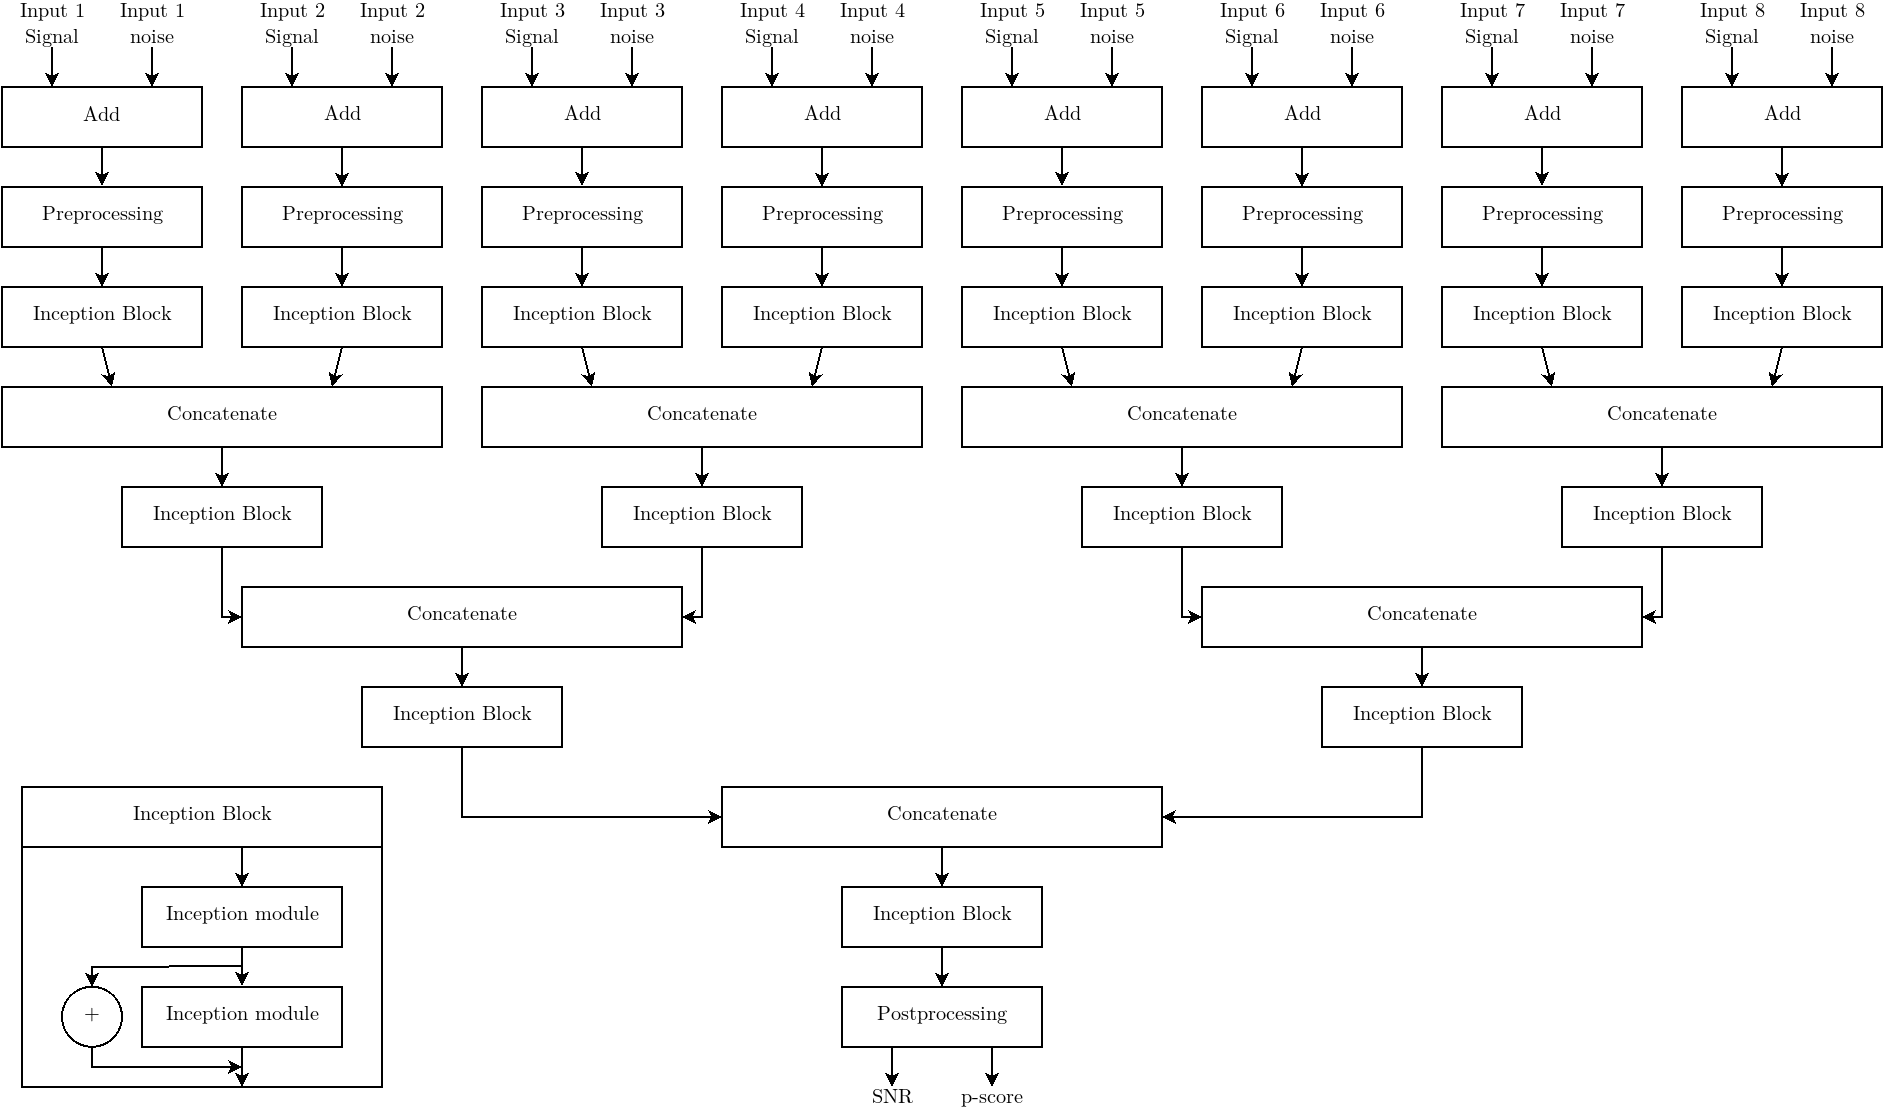
\includegraphics[angle=-90, origin=c, height=0.77\textheight]{collect_inception_res_net_rev_1_version_2.png}
\caption[Cascading architecture of a collect-inception-res network]{The architecture of a cascading collect-inception-res network. The preprocessing layers are shown in \autoref{fig:preprocessing}. The postprocessing layer is shown in \autoref{fig:postprocessing}.}\label{fig:cascade_inception_res_net}
\end{figure}

%\subsubsection{Testing Networks on Corrected Data}

\begin{comment}
Using the corrected data generator with the previously well performing inception-res networks on data, where all previously mentioned parameters were being varied, showed how big the impact of the error was. The sensitivity dropped from 95\% in every \gls{snr} bin to below 20\% in the loudest bin. The collect-inception-res network held up a bit better, dropping to 40\% sensitivity in the loudest bin. From this point we tried to recover some of the lost performance by developing new features and implementing them into the collect-inception-res network.\medskip\\
One of the first tests was training the network to just optimize the p-score rather than both \gls{snr} and p-score, as this second output usually performed a little better than the \gls{snr} output. This did however not work and decreased the performance of the network significantly, reaching only $\sim 12\%$ at the loudest point. Using the original architecture with both outputs but adding in one more inception module per stack also resulted in worse performance overall. This decrease, however, was not quite as significant, dropping only to 30\% in the loudest bin.
\end{comment}

\subsubsection{Testing Alternative Loss Functions and Layers}
After the performance on the difficult data of our networks could not be recovered by simple alterations of the architecture, we decided to try and optimize our algorithm to the specific problem of \gls{gw} detection.\smallskip\\
One of the prominent problems the network has is that estimating pure noise with a large \gls{snr} value significantly decreases sensitivity. An overestimated noise sample is a lot worse than an underestimated signal, as the former has an effect on all \gls{snr} bins. Therefore we tried to implement a loss function that mimics this behavior, by growing exponentially for overestimating noise and only linearly for underestimating it. For signals this behavior is swapped, i.e. the loss grows exponentially for underestimating signals and linearly for overestimating them. The details on how this loss looks like and how it was derived can be found in \autoref{app:custom_loss}. It turned out that this approach also didn't help but rather decreased the sensitivity of the network. It even seemed to push the two categories closer together. Further research in this area might prove useful though.\smallskip\\
We also briefly tried to use a mean average percentage error as loss function for the \gls{snr} output to penalize errors at low values more strongly. The results of this different loss function were mixed but mostly resulted in worse performance.\medskip\\
% (see 21.07.2019 in \cite{network_wiki}). Other tests (e.g. (22.07.2019 (2)) in \cite{network_wiki}) showed similar results.\medskip\\
Another approach we took was close in nature to that of SincNet \cite{sincnet}. SincNet convolves the input data with a parameterized filter, that is used in standard signal processing. This has two main advantages. Firstly, the filters the network applies become more interpretable and thus reveal more insight into what the network is actually trying to accomplish. Secondly, the number of trainable parameters is reduced as we don't need to train a large convolution kernel but rather some parameters of a known function. Their implementation used the parametrized layer only as the first layer of the architecture and showed improvements over other purely convolutional approaches when trying to recognize speakers \cite{sincnet_speach}. Based on this work we used our adaptation only as a first layer, too. Instead of using Sinc-functions, we tried to use sums of sine waves. The convolution kernel is thus given by $\sum_{i=1}^n A_i\cdot\sin\lr{f_i t + \varphi_i}$, where $A_i$, $f_i$ and $\varphi_i$ are learned parameters and $t$ is used to sample the function. The general idea behind this approach is to enable the network to construct a crude template of a general waveform by combining multiple sine waves. To restrict the available frequencies, the layer is given a low and high frequency cutoff. This restriction is necessary to determine the shape of the convolution kernel. To sample a sine wave of frequency $f$, according to Nyquist, one needs to sample at least with a rate of $2f$. Therefore the sample rate is given by $\diff t = \frac{1}{2 f_\text{high}}$. As we want to fit at least one complete cycle of the lowest frequency into our kernel, the number of samples in the kernel is given by $N=\frac{f_\text{low}}{2f_\text{high}}$. By default the convolution kernel will always be filled with samples, e.g. a sine wave of frequency $f=2f_\text{low}$ will manage two full cycles in the convolution kernel. We called this layer ''Wave-Convolution'' or ''WConv1D'' in short and will from here on out refer to it by this name.\\
To get a quick estimate of how well this new approach does we devised a simple network consisting of only two convolution-type layers and two dense layers to get the correct output. We than compare two iterations of this network, one trained with the new Wave-Convolution layer and one using a usual convolutional layer. All other parameters are kept constant. For the convolutional layer, we choose the kernel size in such a way that the number of trainable parameters is on a comparable scale.\\
First tests of this new layer did apply some false windowing and used a skewed methodology. The results produced by these early tests lost out to pure convolutional quite strongly and thus this approach was not further pursued. Revisiting the idea close to finishing this project and fixing the errors previous runs made paints a different but not clear picture. Now the WConv1D layer significantly outperforms the traditional convolutional layer, almost doubling the sensitivity in every bin. The results are however questionable in multiple ways. Firstly, both networks experienced strong overfitting, thus rendering the training almost meaningless. Therefore, the difference in performance may be down to pure chance. Secondly, the networks were only followed by a single convolutional layer before being fed into the final dense layers. The test setup therefore doesn't consider the impact on deep networks. Furthermore, the convolution kernel used for the convolutional network was of size 288, which is well beyond the usual kernel sizes of 16 used in \gls{cnn}s designed for filtering \gls{gw} data. It is thus questionable if the extra effort required would justify the use of a WConv1D layer. Finally, the layer was not compared in state of the art networks derived in \autoref{sec:evolution_convolution} to \autoref{sec:evolution_bad_data}. Therefore, a lot more research would be necessary to determine the use of this new approach.\medskip\\
As no architectural alteration proved to be highly beneficial to the performance of the network for the difficult data where a lot of parameters are varied, we went back to using the data that only varies the \gls{snr}. We than combined the general approach of the \gls{tcin} with the new cascading architecture and found that it outperforms the traditional \gls{tcin}. This combination is the final architecture we tried and will be explained in further detail in \autoref{sec:final_architecture}. We then used this final architecture and trained it on the data described in \autoref{sec:data_generating_process} to finally evaluate it.

\subsubsection{Miscellaneous Findings}
We conclude this section with a few statements about general findings of our research.\\
Using dropout layers in the initial layers after normalizing the input generally had a positive effect on the achievable sensitivities, even when the number of input samples was chosen large enough to avoid overfitting. On the other hand it generally comes with the disadvantage of the loss being a lot more jumpy throughout the training and trends in the loss being washed out.\\
We used the \gls{sgd} variant ''Adam'' as an optimizer for most of our runs and did not see improvements when trying different ones like ''AdaDelta'' or standard \gls{sgd}. We also briefly tried modifying the learning rate but could not improve results, thus staying with the default learning rate of $10^{-3}$.\\
Finally, when training a network and monitoring the sensitivity throughout the training process, we noticed drops to zero sensitivity at some point. These got more frequent as training went on. We hypothesize that this drop is due to the network trying to split noise and signals rather strongly. If one of the noise samples resonates strongly with the network and it ''thinks'' to have seen a signal, it will push the value for this sample higher and higher. The p-score additionally will saturate at 1. We therefore recommend to stop training the network after a few of these dips to 0 sensitivity occurred.


\subsection{Final Network}
\textcolor{blue}{Talk about how the final network looks, how it performs and what could be imporved.}\\
\textcolor{red}{First final network stored at tcn\_collect\_inception\_res\_net\_rev\_6\_248201905643}\\
Trying to optimize a \gls{nn} to a specific task is a problem that has no specified end. Therefore, the architecture discussed in this section is only the best of our current efforts. We will start off by discussing it and the underlying design decisions in detail and afterwards evaluate the performance on a long set of continuous strain data.
\subsubsection{Architecture}\label{sec:final_architecture}
\textcolor{blue}{Explain the architecture and the reasoning behind it. Talk about the size of the model, where it could be trained and what the drawbacks of the architecture are. (Drawbacks: Large memory size (hence small batch size), very deep $\to$ slow training and maybe vanishing gradients, hyper-parameter-optimization is hard, not everywhere are residual connections (fixable by further dimensional reduction))}\\
All illustrations for this section can be found in \autoref{app:illustrations_final_architecture}.\\
The final architecture is a collect-inception-res network with \gls{tcn}s as denoisers for every stack. Each stack is attributed its own sample rate and they cascade down to the two outputs. The first output is supposed to give an estimate of the \gls{snr} of the input data whereas the second one gives a p-score, a value that is used for pure binary classification, i.e. just gives information about whether or not a \gls{gw} is present in the data. To stress again, the p-score is not a probability but just a value that is bounded by 0 and 1 that, when a threshold is applied, gives a binary answer. A high-level overview of the network is shown in \autoref{fig:high_level_final_network}.\\
We will now give a detailed description of each module depicted in \autoref{fig:high_level_final_network}, working our way down from the input. We will only discuss each module once, as all of them share the same parameters.\\
The inputs are labeled 1 to 8, each consisting of an individual input for signal and noise. The order of these inputs is the reversed order of the chopped up time series, i.e. input 1 corresponds to the last \SI{0.5}{\s} of data sampled at \SI{4096}{\hertz}, input 2 is the interval from \SIrange{0.5}{1}{\s} sampled at \SI{4096}{\hertz} and so on. The final input thus is the last \SI{32}{\s} sampled at \SI{64}{\hertz} (for details see \autoref{sec:data_generating_process}). The first layer in each stack simply adds the two stack-inputs for signal and noise together. This sum is then fed to a \gls{tcn}.\\
The \gls{tcn} stacks 11 blocks of dilated convolutional layers with causal connections on top of each other. Every block has a total kernel size of three and the dilation is set to $2^i$, where $i$ is the depth of the \gls{tcn}. Furthermore, each block consists of two stacked convolutional layers with dilation rate $2^i$, each followed by a  batch normalization, ReLU activation and dropout layer. The latter has a dropout rate of 0.1. Finally, the entire block is preceeded by a dimensional reduction layer and wrapped with a residual connection. (see \autoref{fig:tcn_block}) The implementation follows \cite{tcn_paper}, replacing their weight normalization by batch normalization, as Keras does not provide a weight normalization layer. The depth was chosen such that the receptive field of the \gls{tcn} encapsulates all $2048$ input samples.\\
Each of the \gls{tcn} has their own training goal, which is given by the corresponding signal input. The loss for this part is chosen to be \gls{mse} and added to the total loss with a weight factor of $0.1$. The weight is set so low as the \gls{tcn} is not able to reliably recover the waveform from the input data and we don't want the network to try and optimize just the \gls{tcn}s without optimizing the final outputs we care about. With this training goal, the \gls{tcn} is meant to act as a denoiser to the input data. Its output is then added back onto the input, to amplify any signal it found. To avoid throwing away information the \gls{tcn} could not recover, we only amplify the signal and don't just feed the output itself to the following layers.\\
As a next step we do some preprocessing for the following collect-inception-res network. The authors of \cite{inception_module} found that using a few simple convolutional layers before a stack of inception modules helps the network learn. We could verify these findings when testing different inception networks and thus included this preprocessing step. It starts of with a batch normalization layer, followed by a dropout layer with a dropout rate of $0.25$. They are followed by two stacked blocks of convolution, batch normalization and ReLU activation, separated by a max pooling layer with pool size 4. See \autoref{fig:preprocessing} for a visual aid.\\
The main workhorse for the collect-inception-res network are the inception blocks. Each of them contain two stacked inception modules, separated by a batch normalization layer. The second inception module also utilizes a residual connection. The first one could be equipped with a residual connection as well if it was preceded by a  dimensional reduction layer, adjusting the number of channels to $224$. Within the inception modules, we empirically chose the number of filters to be descending for an increasing kernel size. We furthermore found that kernel sizes $(1,2,3)$ work best in these modules. These parameters could probably be optimized even further, but we could not do so in a feasible amount of time. The inception block is depicted in \autoref{fig:inception_block}.\\
All concatenation layers except the final one are furthermore equipped with another auxiliary output that use the \gls{snr} label as a training goal. To reduce each of these layers down to a single value we use a stack of one average pooling layer with pool size 8, one dimensional reduction layer with 16 filters and one final dense layer with a single neuron and a ReLU activation function. The output of the dimensional reduction is flattened to be usable for a dense layer. This action was taken to help against vanishing gradients and was inspired by the architecture of \cite{inception_module}. The loss used is \gls{mse} and is also weighted by $0.1$.\\
The post-processing consists of a max pooling layer with pool size 4, a dimensional reduction layer with 32 filters and, depending on the output, two dense layers with neuron numbers $(2,1)$ for the \gls{snr} output and $(3,2)$ for the p-score output. For the \gls{snr} output we use a ReLU activation function and for the p-score output a softmax activation function. The loss for the \gls{snr} output is \gls{mse} and has a weight of $1$ whereas the p-score output uses a categorical crossentropy as loss and a weight of $0.5$ to have more of an emphasis on the \gls{snr}. The postprocessing step is shown in detail in \autoref{fig:postprocessing}.\medskip\\
This architecture was derived empirically by the process described in \autoref{sec:evolution_of_architecture} as it showed the best performance in regards to the sensitivity on the validation set. The specifics of the performance are discussed in the next section. It does, however, come with multiple drawbacks. The general problem of this architecture is its size and complicated structure. The first obvious complication is the size of necessary video memory. The model takes about \SI{18}{\giga\byte} to train with a mini-batch size of 24. The GPU with the largest memory we could use for a full training run was a NVIDIA Titan V with a capacity \SI{\sim 12}{\giga\byte}. To train this network on such limited memory required us to decrease the mini-batch size to 16. Even though the network just barely fit into memory and Tensorflow stated that additional performance might be gained if more memory was available. This is backed by the GPU utilization that constantly jumped between 20\% and 100\%. Overall each epoch training on the stated $322,500$ sample plus the validation step took \SI{\sim 6}{\hour} to finish.\\
As each epoch takes such a long time, it is very difficult to optimize the hyper parameters, like number of inception modules, kernel sizes within these modules, number of filters in these modules, dropout rate, etc.\\
Finally, a network of this depth is always vulnerable to the vanishing gradient problem. We try to combat this with the auxiliary outputs and their loss functions but cannot rule it out.

\subsubsection{Network Performance}\label{sec:network_performance}
\textcolor{blue}{Evaluate the performance of the network. Show sensitivity curves, talk about speed advantages, how does it in both cases compare to matched filtering? How does it compare to related works? (Reference the BNS-Net paper, what is different between our approach and theirs? Why does theirs seem to work a lot better? Does it?)}
%\textcolor{blue}{Compare the speeds of both methods, the accuracy. What kind of drawbacks does the network have, what are its advantages, how should it be used and understood? (Not as a standalone method of analysis but rather as a starting point for samplers and a quick way of estimate certain properties.)}
To evaluate the performance of the final architecture we use a testing set that contains \SI{4927488}{\s} = \SI{\sim 57}{\day} of continuous data. This data was created independently of the training and validation set and split into 1203 parts of length \SI{4096}{\s}. Each of these parts is evaluated by the trained network, which was described in detail in \autoref{sec:final_architecture}, using a moving window with step size \SI{0.25}{\s} to generate the correct input data format. Therefore, each window is whitened by the analytic \gls{psd} \verb|aLIGOZeroDetHighPower| which is provided by the software library LalSuite \textcolor{red}{[Citation]} and re-sampled. The details on how these processing steps take place are discussed in \autoref{sec:data_generating_process}. The output of this procedure are two time series of duration \SI{4024}{\s} and time resolution \SI{0.25}{\s}. These two time series contain the predicted \gls{snr} and p-score values at each point where a window was evaluated. The difference of \SI{72}{\s} between the input and the output is due to the time span of the window that is used.\\
The testing set contained 37758 injections. They are spaced out to appear every \SI{200}{\s} with the exact position varying by \SI{\pm 20}{\s}, but are not placed within the first or final \SI{256}{\s} of any of the 1203 parts. The source parameters are distributed in the following way: Both component masses are drawn from a uniform distribution between \SIrange{1.2}{1.6}{M_\odot}, the coalescence phase and polarization angle are uniformly distributed within the interval $\left[0,2\pi\right]$ and the inclination is drawn from $\arccos(x)$, where $x$ is uniformly distributed between $-1$ and $1$. We still neglect spins and tidal deformabilities, as both of these effects are expected to be small for astrophysical events \textcolor{red}{[Citation]}. The sky position is distributed volumetrically, meaning that the right ascension is uniformly distributed between $0$ and $2\pi$, the declination is drawn from $\arccos(x)-\pi/2$, where $x$ again is uniformly distributed between $-1$ and $1$, and the distance goes as $r^2$ between \SIrange{0}{400}{\mega\parsec}. The waveforms are generated using the model TaylorF2. All noise is generated using the \gls{psd} \verb|aLIGOZeroDetHighPower| of LalSuite.\smallskip\\
To evaluate the performance of our analysis, we calculate the sensitivity of the search at given false alarm rates. At this point we want to address the comments of \cite{cnn_magiacal_bullet}. They suggest that no statistically meaningful false alarm rate can be derived from a \gls{nn}-based approach that classifies data into the two categories ''noise'' and ''signal''. They hinge their argument on multiple points. Firstly, the network is trained with a certain ratio of examples for signals and for pure noise. False alarm rates derived from the false positive rate on the training/validation set are therefore only applicable if the final distribution of signals within the data is similar to that within the training set. This is however a problem as signals in real data are comparatively rare, whereas for efficient training the ratio of signals to noise should be close to $1:1$. We address this issue by using different ratios in all three sets used for the network. Specifically the training has a ratio of roughly $1:1$, the validation set has a ratio of roughly $3:1$ and the testing set has on average a ratio of $6:194$. The second issue the authors of \cite{cnn_magiacal_bullet} point out is the significance assigned to each detection candidate. In the case of binary classification the output would always be thresholded to yield either $1$ or $0$. Therefore, the false alarm rate assigned to every event would be the same. As we are training for \gls{snr} and p-score, we do have the means of assigning different false alarm rates to different events, as we can determine the false alarm rate at the recovered \gls{snr}. This could however also be done by using the p-score as a ranking statistic. The third point of critique of \cite{cnn_magiacal_bullet} is the use of a sliding window approach and how to treat parts of the output, where the network jumps between claiming a detection and claiming no detection at successive points in time. To get around this issue, we cluster detection candidates into blocks, where the network is confident to have found a signal. If any detection candidates are within \SI{\pm 1}{\s} of another detection candidate they are clustered together and thus believed to belong to the same event. Any times in between are also believed to belong to the event regardless of whether or not they exceed the threshold value that is set to claim detection. To give a single point in time where we believe the event to have taken place, the time that is associated to each cluster is the maximum of either the \gls{snr} or the p-score output. As such we get two sets of detection candidates. We get another one if we only allow detection candidates that exceed the threshold in both ranking statistics. The final issue the authors of \cite{cnn_magiacal_bullet} address is the fact that during training all waveforms are provided to the network at a very specific range in time. They say that \gls{nn}s are known to pick up on such subtle details and thus might not be able to handle waveforms that are not correctly aligned. Therefore a sliding window approach might not be suitable. We think that using a sliding window to generate the results addresses this problem.\smallskip\\
We start the discussion of the new architecture by examining both outputs and their statistics separately We then consider the combination of both outputs and finish this section off by comparing the results to a matched filtering based approach.\\
The false alarm rate of the \gls{snr} output is shown in \autoref{fig:false_alarm_snr}. To use our algorithm to alert astronomers of a \gls{gw} event, we would need to reach false alarm rates of about 1 per 2 month. Evaluating the false alarm rate to \gls{snr} 20 yields a false alarm rate of 38.4 false alarms per month. It is even questionable if the network is capable to reach lower false alarm rates, as some false positives were attributed very high \gls{snr} values. The loudest false positive was assigned a value of 123672.85. One could possibly introduce a high cutoff above which detection candidates are vetoed. Choosing such a cutoff however would need to be done with great care to not veto a lot of loud physical events.\\
We trained the network using waveforms with injection \gls{snr} down to values of $8$. Using this value as a threshold gives a false alarm rate of 107.8. The upper limit for training waveforms was given by \gls{snr} 15. At this value we have a false alarm rate of 44.7. Even though the false alarm rate does improve throughout the range of provided training examples, but not by much if we use the total change as reference. Most of the false alarm are given below the training range. As the high value for the loudest false positive and the overall flatness of the false alarm rate at high \gls{snr}s suggests, the greatest contribution to the false alarm rate comes from very loud glitches. Early tests suggested that these glitches usually exceed the threshold value only for 1 or 2 samples. Therefore, vetoing detection candidates that have high values and exceed the threshold only briefly might improve overall performance. Further careful analysis would be necessary to give a final conclusion.\\
Pure noise samples were attributed a label of \gls{snr} 4. We therefore expect very high false alarm rates at that value. Indeed we get a false alarm rate of 14704.6 at that threshold.\\
Finally we want to compare the false alarm rate of the loudest noise sample from the testing set with its corresponding
\begin{figure}
\centering
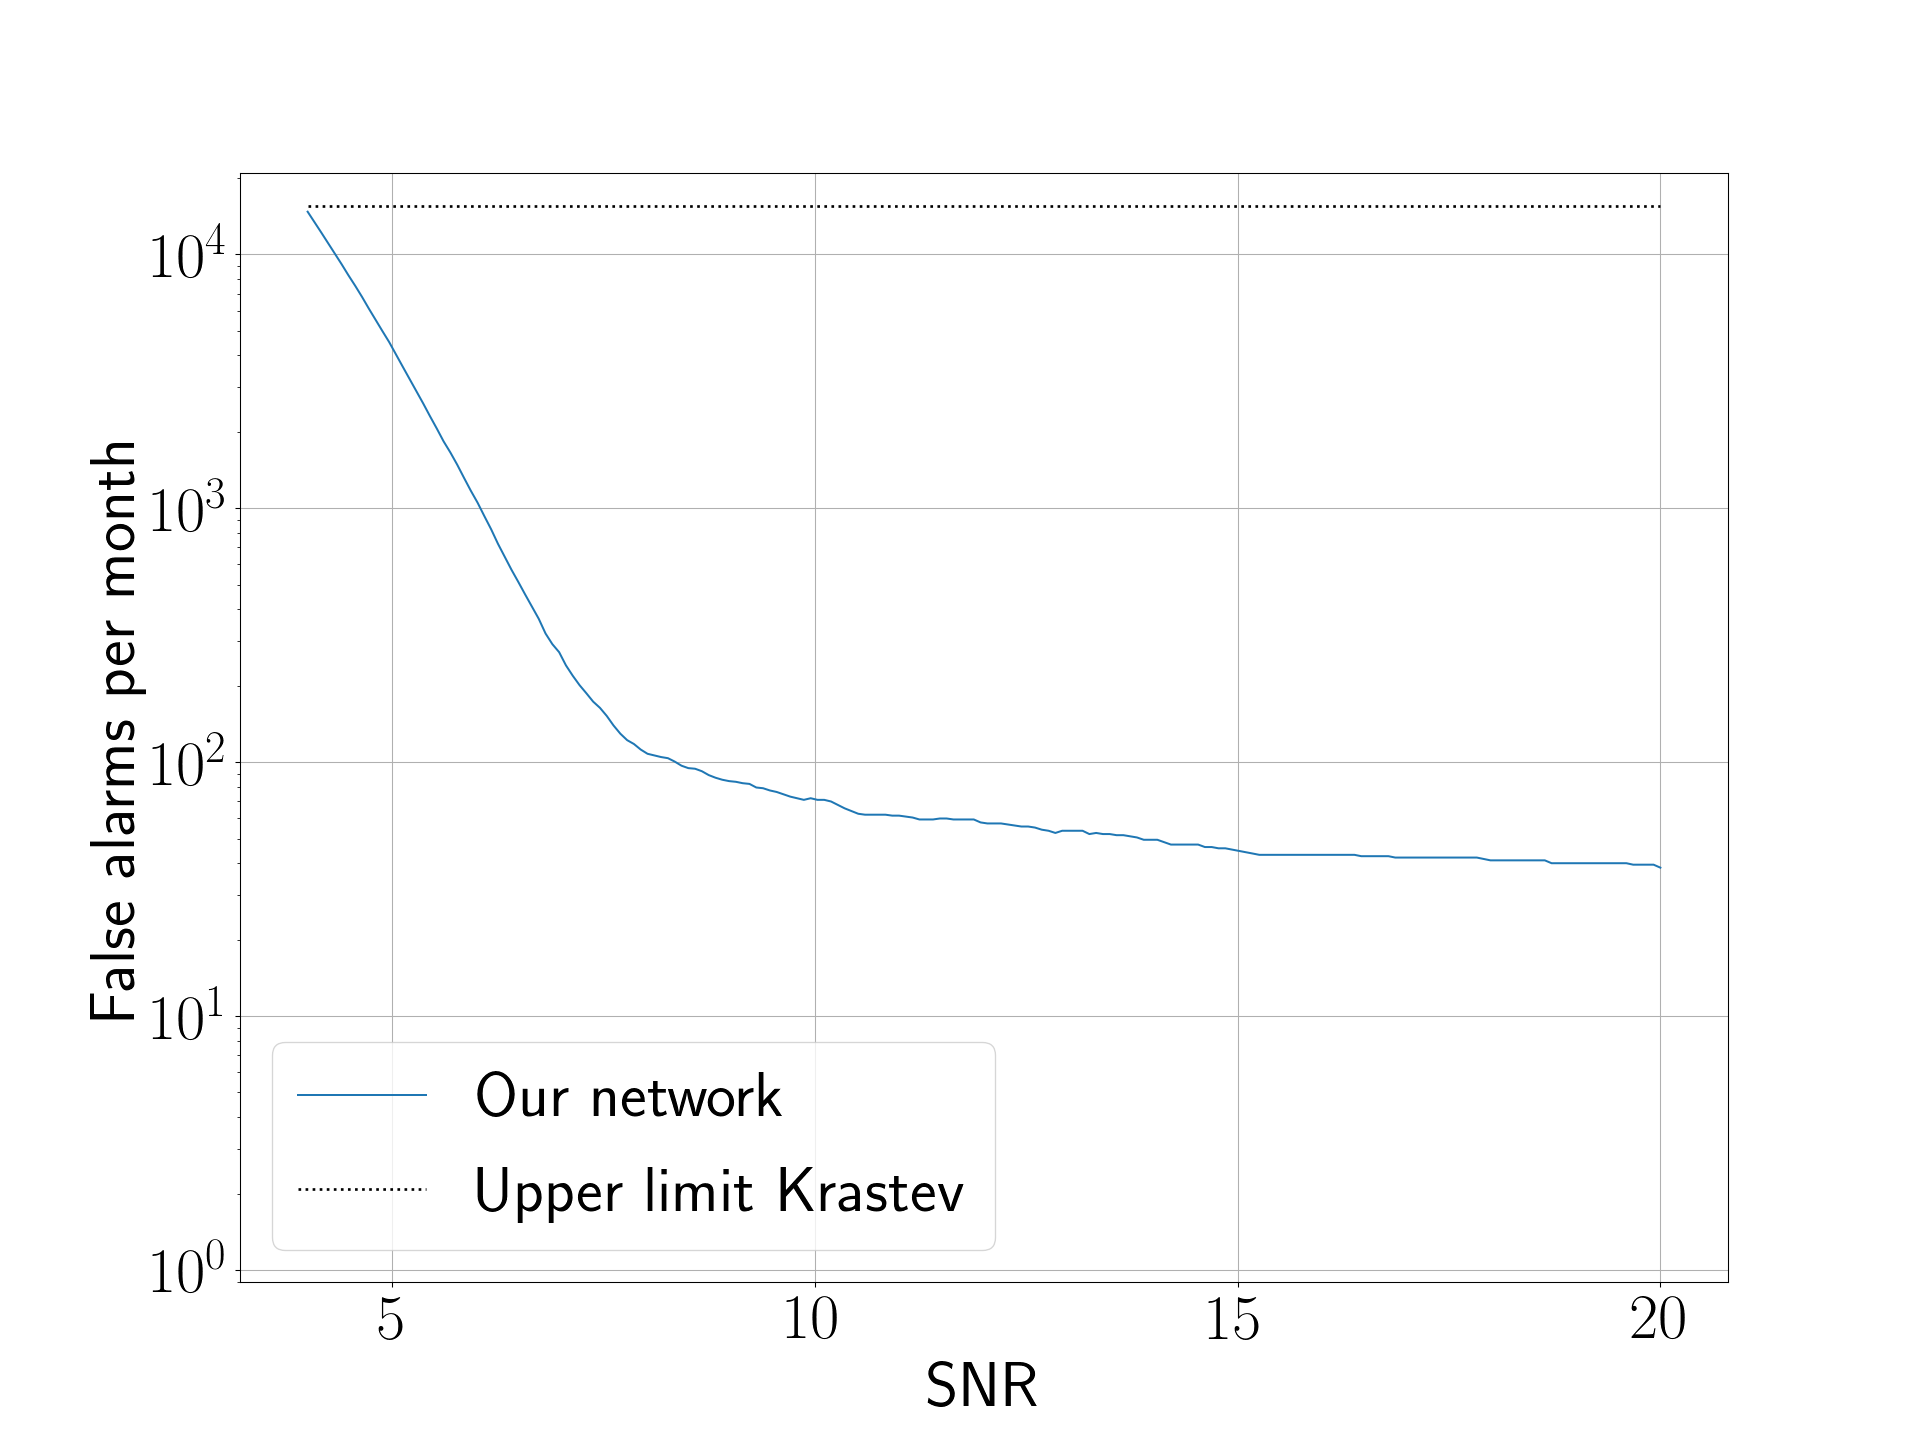
\includegraphics[width=0.75\textwidth]{FalseAlarmSNR.png}
\caption[False alarm rate for SNR]{The false alarm rate given as a function of the recovered \gls{snr} value. The statistics are evaluated on the testing set of duration \SI{4927488}{\s}. At \gls{snr} 20 it reaches a false alarm rate of 38.4 samples per month.}\label{fig:false_alarm_snr}
\end{figure}
\begin{figure}
\centering
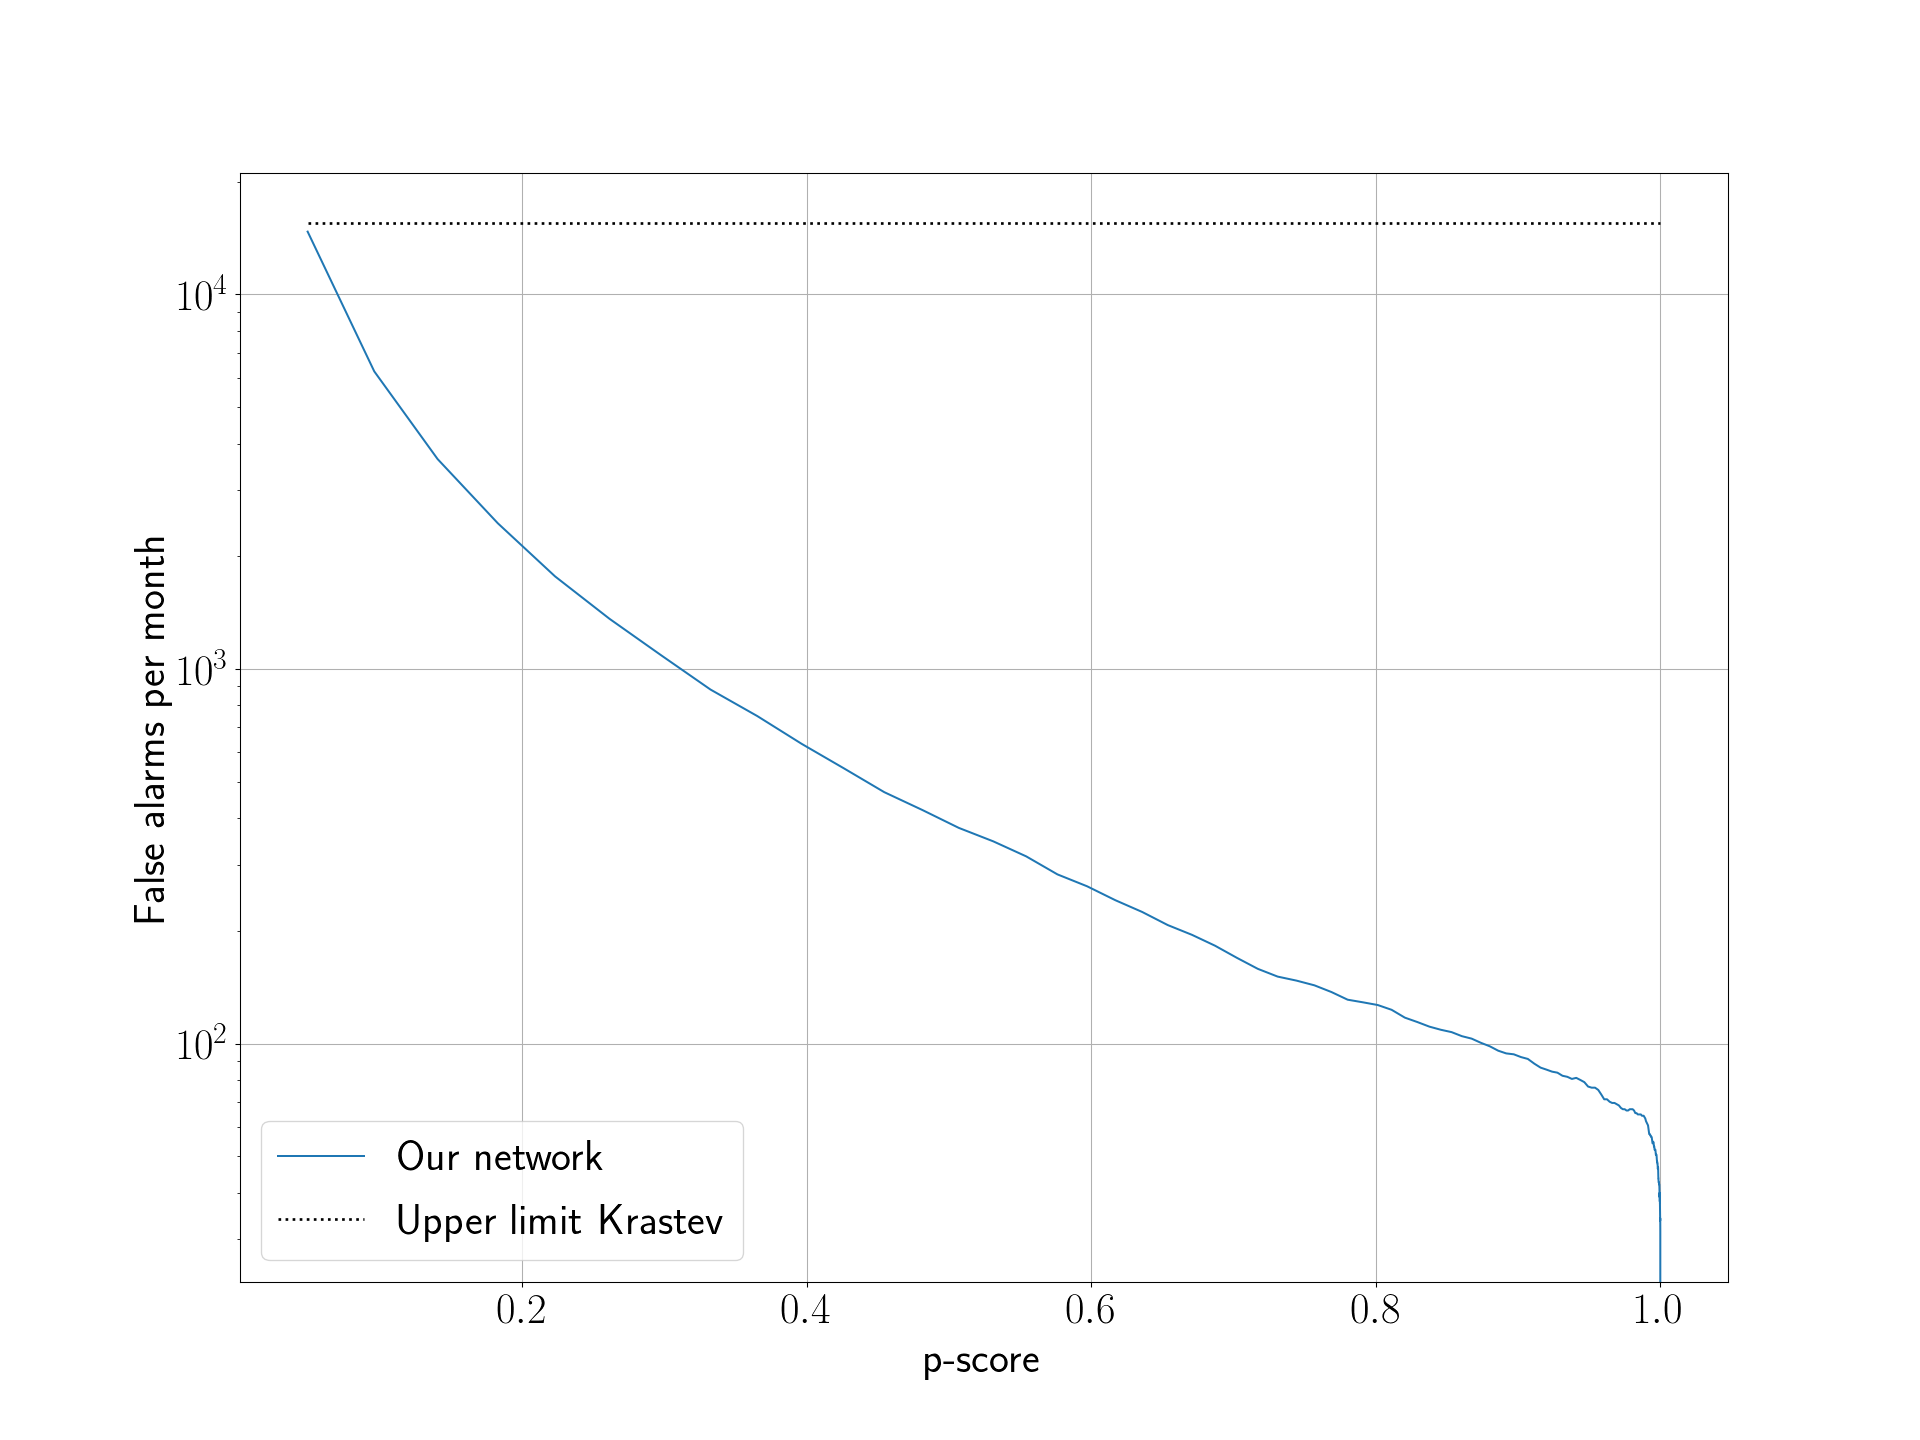
\includegraphics[width=0.75\textwidth]{FalseAlarmP.png}
\caption[False alarm rate for p-score]{The false alarm rate given as a function of the recovered p-score. The statistics are evaluated on the testing set of duration \SI{4927488}{\s}. The false alarm rate drops significantly for values close to 1. At p-score 1 the false alarm rate is expectantly 0. The next smallest sample is at p-score $1-10^-5$ with a false alarm rate of 31.6.}
\end{figure}
